% !TEX TS-program = pdflatex
% !TEX encoding = UTF-8 Unicode

\documentclass[oneside, 11pt]{book} % use larger type; default would be 10pt

\usepackage[utf8]{inputenc} % set input encoding (not needed with XeLaTeX)

%%% Examples of Article customizations
% These packages are optional, depending whether you want the features they provide.
% See the LaTeX Companion or other references for full information.

%%% PAGE DIMENSIONS
\usepackage{geometry} % to change the page dimensions
\geometry{a4paper} % or letterpaper (US) or a5paper or....
\geometry{margin=2.5cm} % for example, change the margins to 2 inches all round
%\geometry{top=2cm, bottom=2cm}
% \geometry{landscape} % set up the page for landscape
%   read geometry.pdf for detailed page layout information

\usepackage[parfill]{parskip} % Activate to begin paragraphs with an empty line rather than an indent

%%% PACKAGES
\usepackage{dsfont} % gives some custom fonts e.g. natural number N
\usepackage{graphicx} % support the \includegraphics command and options
\usepackage{natbib}
\usepackage{booktabs} % for much better looking tables
\usepackage{array} % for better arrays (eg matrices) in maths
\usepackage{paralist} % very flexible & customisable lists (eg. enumerate/itemize, etc.)
\usepackage{outlines}
\usepackage{amsmath}
\usepackage{amssymb}
\usepackage{mathtools}
\usepackage{physics} % physics related commands 
\usepackage{xcolor} % colours :))
\usepackage{listings} % for displaying code nicely
\usepackage{verbatim} % adds environment for commenting out blocks of text & for better verbatim
\usepackage{subfig} % make it possible to include more than one captioned figure/table in a single float
\usepackage{datetime}
\usepackage[hidelinks]{hyperref}
\usepackage{duckuments}

\usepackage{amsthm} % for remarks
\usepackage{chngcntr} % changing the equation counter
\counterwithout{equation}{chapter}

\usepackage{mathtools}
\mathtoolsset{showonlyrefs}

\let\theorem\relax
\newtheorem*{theorem}{Theorem}{\bfseries}
\newtheorem{lemma}{Lemma}{\bfseries}

\bibliographystyle{apalike} % author name and year on references

%%% PACKAGE OPTIONS
\lstset{
  basicstyle=\ttfamily,
  columns=fullflexible,
  numbers=left,
  breaklines=true,
  postbreak=\mbox{\textcolor{red}{$\hookrightarrow$}\space},
  language=Python,
  showspaces=false,
  showstringspaces=false
}

% These packages are all incorporated in the memoir class to one degree or another...

%%% HEADERS & FOOTERS
\usepackage{fancyhdr} % This should be set AFTER setting up the page geometry
\pagestyle{fancy} % options: empty , plain , fancy
\renewcommand{\headrulewidth}{0pt} % customise the layout...
\lhead{}\chead{}\rhead{}
\lfoot{}\cfoot{\thepage}\rfoot{}

%%% SECTION TITLE APPEARANCE
\usepackage{sectsty}
\allsectionsfont{\sffamily\mdseries\upshape} % (See the fntguide.pdf for font help)
% (This matches ConTeXt defaults)

%%% ToC (table of contents) APPEARANCE
\usepackage[nottoc,notlof,notlot]{tocbibind} % Put the bibliography in the ToC
\usepackage[titles,subfigure]{tocloft} % Alter the style of the Table of Contents
\renewcommand{\cftsecfont}{\rmfamily\mdseries\upshape}
\renewcommand{\cftsecpagefont}{\rmfamily\mdseries\upshape} % No bold!

%% CUSTOM COMMANDS
\newcommand{\qb}[1]{\left[#1\right]}
\newcommand{\inte}[4]{\int^{#1}_{#2} #3 \dd{#4}}
\newcommand{\ieval}[3]{\Big[ #3 \Big]^{#1}_{#2}}
\newcommand{\I}[1]{I^2_{#1}}
\newcommand{\al}{\alpha}
\newcommand{\p}{\phi}
\newcommand{\codeword}[1]{\texttt{\textcolor{black}{#1}}}
\newcommand{\ds}{\dots}
\newcommand{\T}[1]{T_{#1}(z)}
\renewcommand{\l}{\lambda}

%%% END Article customizations

\title{The Hydrodynamic Stability of Viscous Plane Flow}
\author{Oscar Rummery}

\begin{document}
\frontmatter

\maketitle

\newpage

\section*{\centering Declaration}
\begin{center}
    \emph{This piece of work is a result of my own work except where it forms an assessment based on group project work. In the case of a group project, the work has been prepared in collaboration with other members of the group. Material from the work of others not involved in the project has been acknowledged and quotations and paraphrases suitably indicated.}
\end{center}

\section*{\centering Acknowledgements}
\begin{center}
    \emph{I'd like to thank my project supervisor, Dr Laura Currie for her encouragement and guidance throughout this project.}
\end{center}

\newpage

\tableofcontents

\newpage

\mainmatter

\chapter{Introduction}
\label{chap:intro}
\section{Hydrodynamic Stability and Parallel Shear Flows}
What is hydrodynamic stability? Hydrodynamic stability is the area of fluid mechanics associated with the stability of flows or systems of flow. For virtually any system where a fluid is in motion, hydrodynamic stability is something that must be considered. This includes obvious examples such as rivers or pipes, but also less obvious examples such as blood flowing through vessels.

We see an example of hydrodynamic stability almost every day when we go to turn on a tap. In some cases, the stream of water appears completely clear. This is an example of \emph{laminar flow} and is a visual example of a stable flow. In other cases, possibly even if we change how far we turn the handle / open the same tap (i.e. change the speed at which the water leaves the tap), the stream appears 'cloudy'. This is an example of unstable or \emph{turbulent flow} and appears when the velocity profile of the stream isn't stable. Different taps will display this behaviour at different points when they are turned. This is due to their nozzles having different shapes and also having water flowing through them at different speeds. This nicely demonstrates the impact that changing the velocity and also the channel shape of a flow can have on the stability of a flow. Figure \ref{fig:tapflow} shows an example of a tap producing a stable flow (left) versus an unstable flow (right).

\begin{figure}[h!]
    \centering
    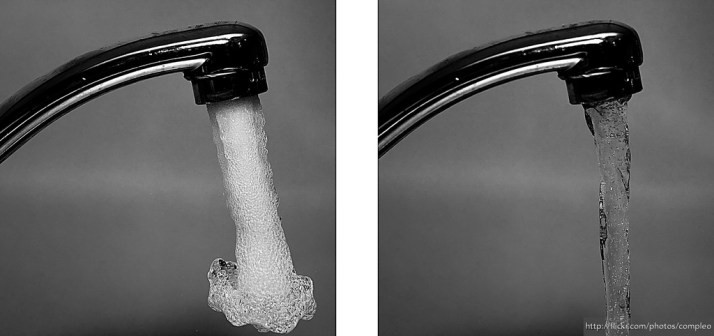
\includegraphics[width=13cm, keepaspectratio]{figures/StablevUnstable.jpg}
    \caption{Turbulent flow versus stable laminar flow from a tap (\href{https://www.flowvis.org/2018/01/30/7640/}{\textcolor{blue}{Image source})}}
    \label{fig:tapflow}
\end{figure}

Another property of a fluid that affects its stability is \emph{viscosity}. In the example of a tap, the most common fluid present is water which has a very low viscosity. However, if it was something like oil or syrup leaving the tap the viscosity is much higher. Figure \ref{fig:viscousflow} shows a number of fluids of increasing viscosity being poured from identical test tubes. How does this affect stability? From what we see in real life, we'd expect viscosity to have a stabilising effect since a fluid like vegetable oil or honey seems a lot more stable when poured than water. The fluids in Figure \ref{fig:viscousflow} seem to show this too, with the least viscous fluid on the left looking more unstable that the more viscous fluids on its right.

\begin{figure}[h!]
    \centering
    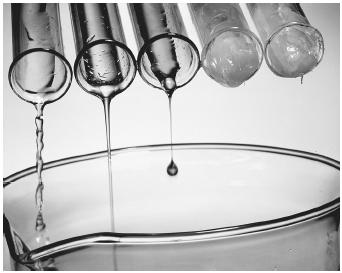
\includegraphics[width=80mm]{figures/viscosity-liquids.jpg}
    \caption{Fluids of increasing viscosity being poured from test tubes. The least viscous fluid is on the left and the most viscous fluid is on the right. (\href{https://schoolworkhelper.net/what-is-viscosity-application-flow-factors/}{\textcolor{blue}{Image source})}}
    \label{fig:viscousflow}
\end{figure}

A parallel shear flow is an axisymmetric flow with parallel streamlines. A plane flow is a 2-dimensional flow i.e. the flow is occurring only in one plane e.g. the $(x, z) $ plane. This report aims to determine the stability of 2-dimensional viscous parallel shear flows, otherwise known as viscous plane flows. 

The most common real-life example of this flow is that of a flow where a fluid is flowing through a pipe or other channel (such as a river bed). This is an important concern in the real world, due to the fact that energy equivalent to roughly 10\% of the world's electricity is used moving fluids through pipes. A significant source of additional cost is turbulence since it involves the fluid swirling around itself and therefore not taking the most efficient path through the pipe. Figure \ref{fig:pipeflow} shows a comparison between turbulent flow (top) and stable flow (bottom) in a pipe. 

\begin{figure}[h!]
    \centering
    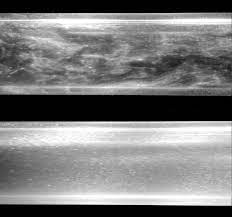
\includegraphics[width=80mm]{figures/pipe_turb.jpg}
    \caption{Turbulent pipe flow (top) versus stable pipe flow (bottom) - (\href{https://www.pumpindustry.com.au/research-reveals-better-manage-turbulence-in-pipes/}{\textcolor{blue}{Image source})}}
    \label{fig:pipeflow}
\end{figure}

In the inviscid case, there are many known analytic results on the stability of parallel shear flows such as \emph{Rayleigh's inflexion point theorem} \citep{rayleigh1880stability} which states that a necessary condition for instability is that the velocity profile contains an inflexion point. 

However, in the viscous case, the analytic results are far less concrete. Some do exist, such as the bounds found by \citet{synge1938hydrodynamical, pai1954generalization} and \cite{joseph1968eigenvalue, joseph1969eigenvalue}, but as will be shown, they are extremely approximate, and do not tell us much about the stability of a specific flow. For this reason, numerical methods are often used instead. The aim of this report is to demonstrate both these analytic results on stability and a numerical method that can be used to more accurately determine the stability of the flow. 

\section{Outline of this report}
Chapter \ref{chap:governing} will introduce the basic state and governing equations for viscous plane flows, along with the family of flows that we are studying, plane Poiseuille and plane Couette flow. The chapter will then turn to manipulating these governing equations, reducing them to just a single equation, the Orr-Sommerfeld equation. The Orr-Sommerfeld equation is an extremely significant equation when studying the linear stability of viscous parallel shear flows, and will be the equation that this report will use to provide both numerical and analytical results on stability.

Chapter \ref{chap:suffcons} contains a discussion on how the Orr-Sommerfeld equation derived in Chapter \ref{chap:governing} can be used to determine whether a flow is stable or not, before deriving separate equations for both the real and imaginary parts of the eigenvalue. We then turn to derive bounds on the real part of the eigenvalue, otherwise known as the wave speed. We derive bounds as seen in \citet{pai1954generalization, joseph1968eigenvalue} which restrict the eigenvalues to a strip in the complex plane. We then derive bounds on the imaginary part of the eigenvalue, deriving the bounds found by \citet{synge1938hydrodynamical, joseph1968eigenvalue, joseph1969eigenvalue}. This gives us two bounds on the stability of a flow and allows us to get an analytic estimate of the critical Reynolds number of Couette and Poiseuille flow. However, these are extremely inaccurate, causing us to seek out a numerical method.

Chapter \ref{chap:numerics} turns to a numerical method to determine the stability of a flow. The numerical methods in question involve the use of Chebyshev polynomials and are referred to as the Chebyshev Tau methods. In the Chebyshev Tau method, we expand our function in terms of Chebyshev polynomials and represent the coefficients of this expansion in a vector. To represent the derivatives we use a matrix that transforms the coefficients of our expansion vector. This produces a matrix system that allows us to determine whether a flow is stable based on its eigenvalues. In the Tau method, the eigenvectors are the coefficients of the Chebyshev polynomial expansion representing our eigenfunctions. This chapter features 3 different ways of forming the generalised eigenvalue problem that we solve in Python, each using a larger system of lower-order differential equations. The reason we perform this split is to reduce the numerical error associated with the extremely large values present in the matrices we are using. This chapter will also explain which eigenvalue algorithm will be used to solve the generalised eigenvalue problems generated by each of our problems.

The numerical results of these methods are discussed in Chapter \ref{chap:results}, followed by a comparison and discussion of the methods used and their advantages and disadvantages. The first set of results shown will be for the case of plane Poiseuille flow, but the chapter will then turn to discuss the results for the case of plane Couette flow. This chapter then turns to show several other key numerical results that we can get from our programs, such as the eigenfunctions (and associated streamfunctions) and the critical Reynolds number. 



\include{chapters/governing}

% \chapter{Viscous Plane Flows}
\label{chap:viscousplane}
This report is focused on \emph{viscous plane flows}. A plane flow is a 2 dimensional flow represented by a velocity profile $ U $ in a single direction. For this project, we will consider $ U $ that are functions of $ z $ only and act in the $ x $ direction. Moreover, our flow will be bounded between $ z = z_{1_*} $ and $ z = z_{1_*} $. Figure \ref{fig:pflow} shows the system we will be analysing in an initial stable state. 

\begin{figure}[htb!]
    \centering
    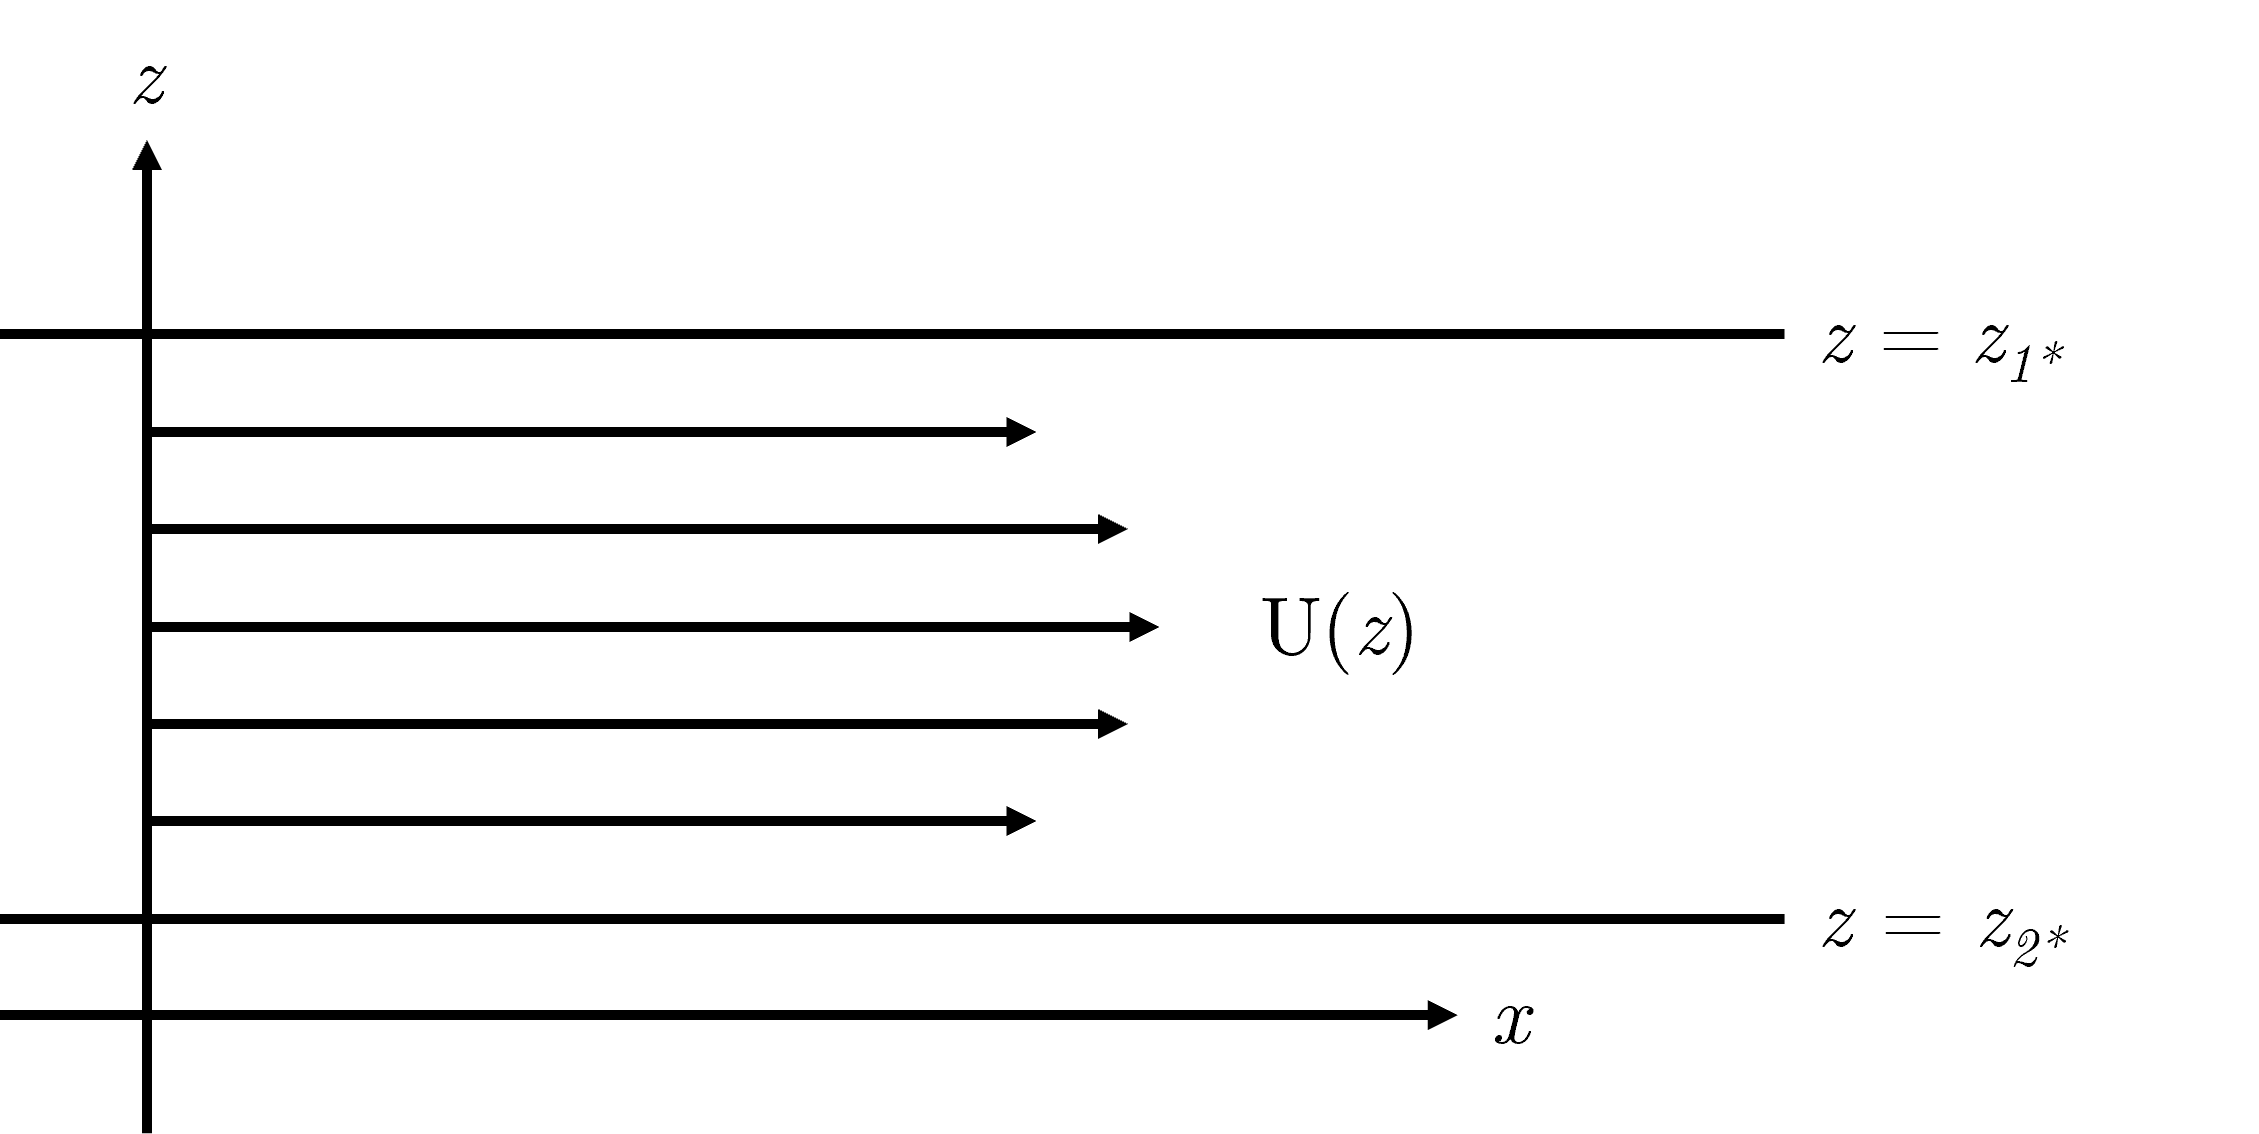
\includegraphics[width=10cm]{figures/PSF.png}
    \caption{The setup of our flow}
    \label{fig:pflow}
\end{figure}

\section{Basic state and governing equations}
\textbf{check the notation used for the dimensional v dimensionless cases, make sure it is consistent}

The fluid discussed in this report is considered to have a constant density i.e. $ \rho = \text{const.} $

Let us use the basic steady flow as defined in \citet{drazin2004hydrodynamic} with the form
\begin{equation}
    \mathbf{U}_* = U_* (z_*) \mathbf{i} \hspace{10px} (z_{1_*} \leq z_* \leq z_{2_*}),
\end{equation}
and boundaries on $z_* = z_{1_*} \text{and } z_{2_*}$ that are either \emph{rigid} or \emph{free}:
\begin{itemize}
    \item \emph{rigid} - normal component of velocity must vanish
    \item \emph{free} - pressure must be constant
\end{itemize}

For this flow, we have the following governing equations that must be satisfied:
\begin{align}
    \div{\mathbf{u_*}} &= 0, \nonumber\\
    \pdv{\mathbf{u_*}}{t_*} + \mathbf{u_*} \cdot \nabla \mathbf{u_*} &= - \frac{1}{\rho} \nabla p_* + \nu \Delta \mathbf{u_*}.
\label{dimgoveq}
\end{align}
These equations are the continuity equation and Navier-Stokes equation for an incompressible fluid respectively. Note that we denote the \emph{kinematic viscosity} $ \nu = \frac{\mu}{\rho} $ and have also set $ f = 0 $ in the Navier-Stokes equation, assuming there is no force acting on the fluid.

\section{Deriving the dimensionless form of our governing equations}
To write the governing equations in terms of dimensionless quantities we utilise the following change of variables. We begin by defining
\begin{align}
    V &= \text{max}_{z_* \in [z_{1_*}, z_{2_*}]} |U_* (z_*)|, \nonumber\\
    L &= \frac{1}{2}(z_{2_*} - z_{1_*})
\end{align}
We will refer to $ V $ as the \emph{characteristic velocity} and $ L $ as the \emph{characteristic length}. Now change our other variables to their dimensionless forms
\begin{align}
    t = \frac{t_* V}{L},\ \mathbf{x} &= \frac{\mathbf{x_*}}{L},\ \mathbf{u} = \frac{\mathbf{u_*}}{V},\ p = \frac{p}{\rho V^2}, \nonumber\\ \mathbf{U} &= \frac{\mathbf{U_*}}{V} \equiv U(z) \mathbf{i} 
\end{align}
We can use this transformation to find dimensionless forms of the various derivatives in the governing equations. By the chain rule we have
\begin{equation}
    \pdv{\mathbf{u}}{t} = \pdv{\mathbf{u}}{\mathbf{u_*}} \pdv{\mathbf{u_*}}{t_*} \pdv{t_*}{t} = \frac{L}{V^2} \pdv{\mathbf{u_*}}{t_*} \implies \pdv{\mathbf{u_*}}{t_*} = \frac{V^2}{L} \pdv{\mathbf{u}}{t},
\label{dut*}
\end{equation}
and
\begin{gather}
    (\nabla \mathbf{u_*})^\mu = \pdv{\mathbf{u_*}}{{x_*}^\mu} = \pdv{\mathbf{u_*}}{\mathbf{u}} \pdv{\mathbf{u}}{x^\mu} \pdv{x^\mu}{{x_*}^\mu} = \frac{V}{L} \pdv{\mathbf{u}}{x^\mu} = \frac{V}{L} (\nabla \mathbf{u})^\mu \nonumber\\
    \implies \nabla \mathbf{u_*} = \frac{V}{L} \nabla \mathbf{u}.
\label{gradu*}
\end{gather}

\textbf{the below needs updating i think or some explanation of what is being done here}

Similarly
\begin{gather}
    (\Delta \mathbf{u_*})^\mu) = \pdv{{x_*}^\mu} (\nabla \mathbf{u_*})^\mu = \frac{1}{L} \pdv{x^\mu}(\frac{V}{L} (\nabla \mathbf{u})^\mu) = \frac{V^2}{L} (\Delta \mathbf{u})^\mu \nonumber\\
    \implies \Delta \mathbf{u_*} = \frac{V^2}{L} \Delta \mathbf{u},
\label{lapu*}
\end{gather}
and
\begin{gather}
    \div{\mathbf{u_*}} = \pdv{{u_*}^\mu}{{x_*}^\mu} = \frac{V}{L} \pdv{u^\mu}{x^\mu} = \frac{V}{L} \div{\mathbf{u}}.
\label{divu*}
\end{gather}
Finally, for $ p_* $ we need just $ \nabla p_* $ in terms of $ \nabla p $, again using the chain rule we obtain
\begin{gather}
    (\nabla p_*)^\mu = \pdv{p_*}{{x_*}^\mu} = \pdv{p_*}{p} \pdv{p}{x^\mu} \pdv{x^\mu}{{x_*}^\mu} = \rho V^2 \pdv{p}{x^\mu} \frac{1}{L} = \frac{\rho V^2}{\mu} \pdv{p}{x^\mu} \nonumber\\
    \implies \nabla p_* = \frac{\rho V^2}{L} \nabla 
\label{gradp*}
\end{gather}
We can now substitute these results into our governing equations \eqref{dimgoveq} to get their dimensionless forms. For the \emph{continuity equation} we use equation \eqref{divu*} to get
\begin{gather}
    0 = \div{\mathbf{u_*}} = \frac{V}{L} \div{\mathbf{u}} \implies \div{\mathbf{u}} = 0.
\end{gather}
Substituting our remaining equations \eqref{dut*}, \eqref{gradu*}, \eqref{lapu*}, \eqref{gradp*} into the \emph{Navier-Stokes equation} we get
\begin{align}
        \pdv{\mathbf{u_*}}{t_*} + \mathbf{u_*} \cdot \nabla \mathbf{u_*} &= - \frac{1}{\rho} \nabla p_* + \nu \Delta \mathbf{u_*} \nonumber\\
        \implies \frac{V^2}{L} \pdv{\mathbf{u}}{t} + (V \mathbf{u}) \cdot (\frac{V}{L}\nabla \mathbf{u}) &= - \frac{1}{\rho} (\frac{\rho V^2}{L} \nabla p) + \nu (\frac{V}{L^2} \Delta \mathbf{u}) \nonumber\\
        \implies \frac{V^2}{L} \pdv{\mathbf{u}}{t} + \frac{V^2}{L} \mathbf{u} \cdot \nabla \mathbf{u} &= -\frac{V^2}{L} \nabla p + \frac{\nu V}{L^2} \Delta \mathbf{u} \nonumber\\
        \implies \pdv{\mathbf{u}}{t} + \mathbf{u} \cdot \nabla \mathbf{u} &= -\nabla p + \frac{\nu}{V L} \Delta \mathbf{u}
\end{align}
Notice that $ \frac{V L}{\nu} $ is the famous \emph{Reynold's number} $ R $. Using this in the Navier-Stokes equation leaves us with our pair of \emph{dimensionless governing equations}
\begin{align}
    \div{\mathbf{u}} &= 0, \nonumber\\
    \pdv{\mathbf{u}}{t} + \mathbf{u} \cdot \nabla \mathbf{u} &= -\nabla p + R^{-1} \Delta \mathbf{u}.
\label{dlessgoveq}
\end{align}

Substituting $ \mathbf{u}(\mathbf{x}, t) = U(z) \mathbf{i} $, $ p (\mathbf{x}, t) = $ into \eqref{dlessgoveq}, we find that $ U(z) $ must satisfy the following equation of motion 
\begin{equation}
    \dv[2]{U}{z} = R \dv{P}{x}
\end{equation}
which limits our choices of $ U (z) $. There are two main important cases defined as follows:
\begin{list}{$-$}{\leftmargin=1cm}
    \item \emph{Poiseuille flow}: $ U(z) = 1 - z^2 $ with $ \dv{P}{x} = const. $
    \item \emph{Couette flow}: $ U(z) = z $ with $ P = const. $
\end{list}

Schematic diagrams for these 2 flows can be seen in Figure \ref{fig:pandcflow}. This leaves us with a family of flows to analyse formed by a linear combination of these 2 types of flow.

\textbf{discuss where these may occur in the real world?}

\begin{figure}[htb!]
    \centering
    \subfloat[Poiseuille flow]{
    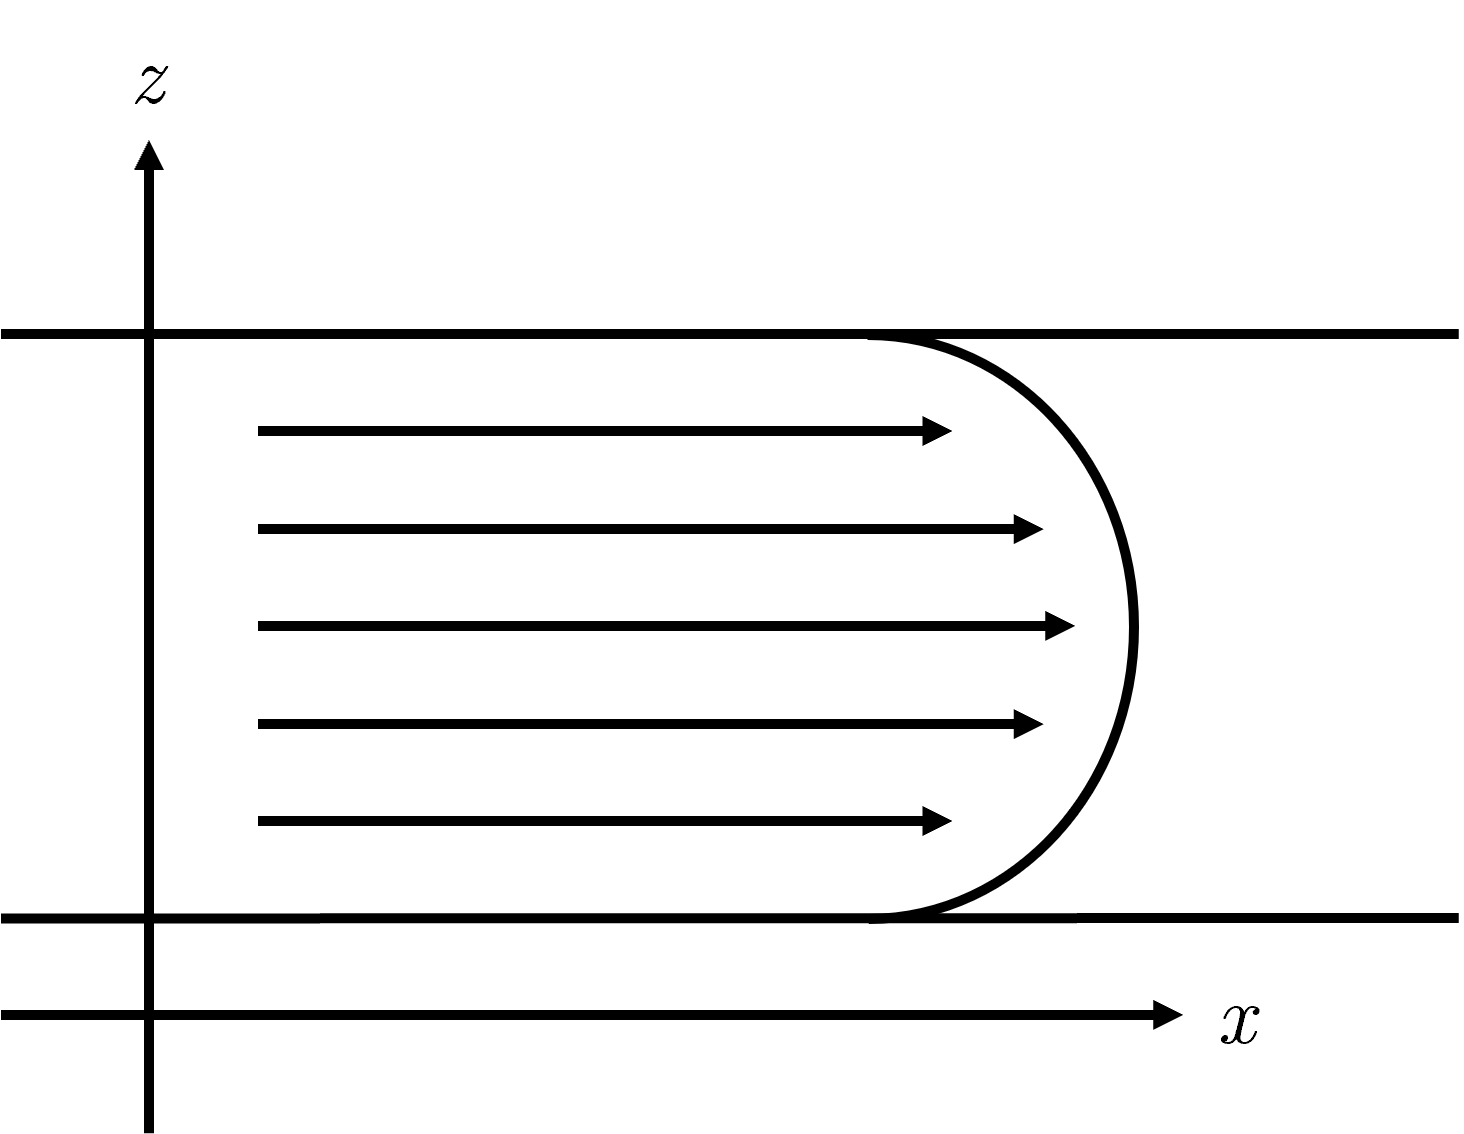
\includegraphics[width=80mm]{figures/PoiseuilleFlow.png}
    }
    \subfloat[Couette flow]{
    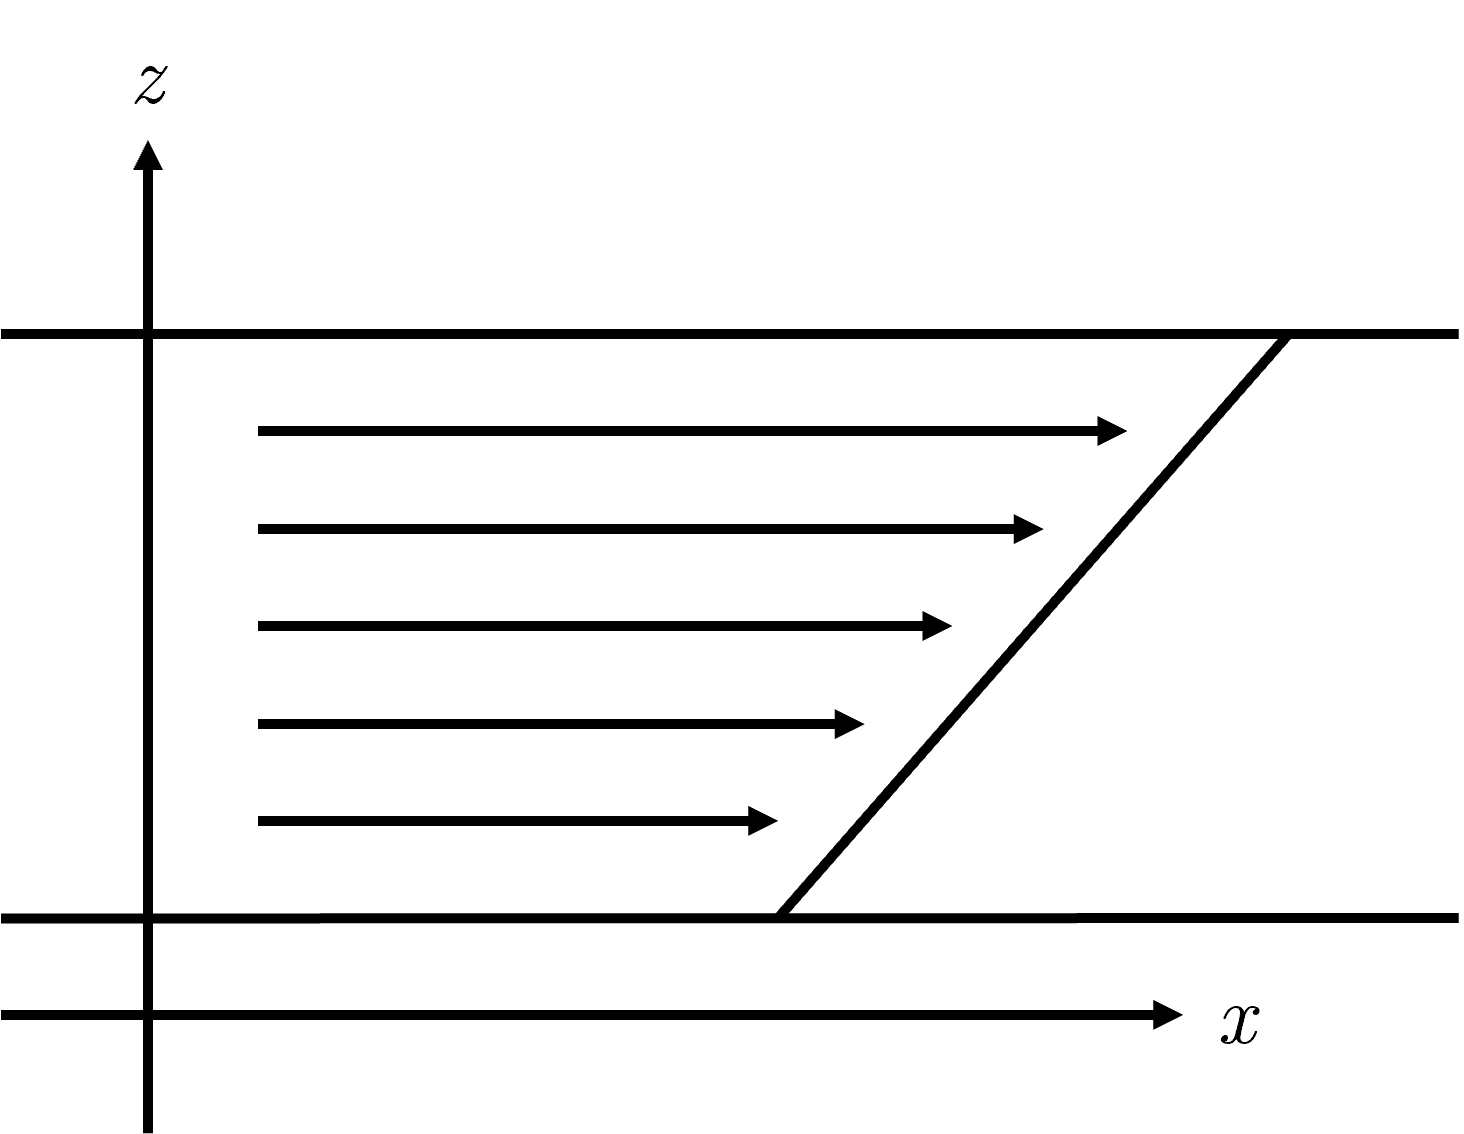
\includegraphics[width=80mm]{figures/CouetteFlow.png}
    }
    \caption{Schematics of plane Poiseuille and plane Couette flow}
    \label{fig:pandcflow}
\end{figure}






% \chapter{Deriving the Orr-Sommerfeld equation}
\label{chap:oseq}
This section derives the Orr-Sommerfeld equation and the results leading to it by linearisation of the governing equations for viscous flow and the use of a stream function solution. The derivation will largely follow the format and processes set out in \citet{drazin2004hydrodynamic} with details and working filled in.

\section{Linearising the governing equations}
We can linearise these equations by writing 
\begin{align}
    \mathbf{u}(\mathbf{x}, t) &= U(z) \mathbf{i} + \mathbf{u}'(\mathbf{x}, t), \nonumber\\
    p(\mathbf{x}, t) &= const. + p'(\mathbf{x}, t)
\end{align}

\textbf{need to double check the ansatz used for P here}

and discarding any terms that are non-linear in $ \mathbf{u}' $ or  $ p' $.
Substituting these forms into \eqref{dlessgoveq} will allow us to find the linearised forms of our governing equations. For the continuity equation, we get
\begin{equation}
    0 = \div{\mathbf{u}} =  \div{( U \mathbf{i} + \mathbf{u}'(\mathbf{x}, t))} = \div{\mathbf{u}'}
\label{contlin}
\end{equation} 
where the term $ \div{U \mathbf{i}} $ vanishes as $ U $ is a function of $ z $ only.
For the Navier-Stokes equation, we linearise the various necessary results separately for readability. 

For $ \pdv{\mathbf{u}}{t} $, 
\begin{equation}
    \pdv{\mathbf{u}}{t} = \pdv{}{t} (U(z) \mathbf{i} + \mathbf{u}'(\mathbf{x}, t)) = \pdv{\mathbf{u}'}{t}.
\end{equation}
Similarly
\begin{align}
    \mathbf{u} \cdot \nabla \mathbf{u} &= (U \mathbf{i} + \mathbf{u}' (\mathbf{x}, t)) \cdot \nabla (U \mathbf{i} + \mathbf{u}' (\mathbf{x}, t)) \nonumber\\
    &= (U \mathbf{i} + \mathbf{u}' (\mathbf{x}, t)) \cdot (\nabla \mathbf{u}' + \nabla U) \nonumber\\
    &= U \mathbf{i} \cdot \nabla \mathbf{u}' + \mathbf{u}' \cdot \nabla \mathbf{u}' + \mathbf{u}' \nabla U \mathbf{i} + U \mathbf{i} \cdot \nabla U \mathbf{i}.
\end{align}
We now omit $ \mathbf{u}' \cdot \nabla \mathbf{u}' $ as it is quadratic in $ \mathbf{u}' $, and by letting $ \mathbf{u}' = (u', v', w') $ we are left with
\begin{equation}
    \mathbf{u} \cdot \nabla \mathbf{u} = U \pdv{\mathbf{u}'}{x} + w' \frac{\text{d}U}{\text{d}z} \mathbf{i}.
\end{equation}
For the right-hand side we get
\begin{align}
    \nabla p &= \nabla (const. + p') = -\nabla p', \nonumber\\
    \Delta \mathbf{u} &= \Delta (U \mathbf{i} + \mathbf{u}' (\mathbf{x}, t)) \nonumber\\
    &= \div{\nabla (U \mathbf{i} + \mathbf{u}' (\mathbf{x}, t))} \nonumber\\
    &= \div{\nabla \mathbf{u}'} = \Delta \mathbf{u}'.
\end{align}
We can now substitute these into the Navier-Stokes equation to get its linearised form:
\begin{equation}
    (\pdv{}{t} + U \pdv{}{x}) \mathbf{u}' + w' \frac{\text{d}U}{\text{d}z} \mathbf{i} = - \nabla p' + R^{-1} \Delta \mathbf{u}'
\label{nslin}
\end{equation}

\section{Normal mode analysis of our linearised equations}
Consider as in \citet{drazin2004hydrodynamic} the normal mode ansatz
\begin{align}
    \mathbf{u}' ( \mathbf{x}, t) &= \hat{\mathbf{u}}(z) \exp{i(\alpha x + \beta y - \alpha c t)}, \nonumber\\
    p'(\mathbf{x}, t) &= \hat{p}(z) \exp{i(\alpha x + \beta y - \alpha c t)}.
\label{osansatz}
\end{align}
This ansatz is derived from the fact that the coefficients in our linearised equations \eqref{contlin} and \eqref{nslin} are only dependent on $ z $. In this ansatz $ \al$, $ \beta$ are the \emph{wavenumbers} of the mode and can take any real value greater than $0 $, and $ c $ denotes the \emph{phase speed} and is a complex number. The value of the phase speed is very important when it comes to analysing the stability of a flow. More details of this will be discussed in Chapter \ref{chap:suffcons}.

As before we let $ \hat{\mathbf{u}} = ( \hat{u}, \hat{v}, \hat{w} ) $.

We now substitute our ansatz \eqref{osansatz} into our linearised governing equations \eqref{contlin} and \eqref{nslin} which gives us
\begin{gather}
    0 = \div \mathbf{u}' = \div \hat{\mathbf{u}}(z) \exp{i(\alpha x + \beta y - \alpha c t)} \nonumber\\
    = i \alpha \hat{u} \exp{i(\alpha x + \beta y - \alpha c t)} + i \beta \hat{v} \exp{i(\alpha x + \beta y - \alpha c t)} + \frac{\text{d}\hat{w}}{\text{d}z} \nonumber\\
    = (i(\alpha \hat{u} + \beta \hat{v}) + \frac{\text{d}\hat{w}}{\text{d}z})\exp{i(\alpha x + \beta y - \alpha c t)} \nonumber\\
    \implies i(\alpha \hat{u} + \beta \hat{v}) + \frac{\text{d}\hat{w}}{\text{d}z} = 0.
\label{os1}
\end{gather}
For the left-hand side of the Navier-Stokes equation, we get
\begin{gather}
    (\pdv{}{t} + U \pdv{}{x}) \mathbf{u}' + w' \frac{\text{d}U}{\text{d}z} \mathbf{i} = -i \alpha c \mathbf{u}' + i \alpha U \mathbf{u}' + \frac{\text{d}U}{\text{d}z} \hat{w} \mathbf{i} \nonumber\\
    = (i \alpha ( U - c) \hat{\mathbf{u}} + \frac{\text{d}U}{\text{d}z} \hat{w} \mathbf{i} \exp{i(\alpha x + \beta y - \alpha c t)},
\end{gather}
and for the right-hand side we get
\begin{gather}
    -\nabla p' + R^{-1} \Delta \mathbf{u}' = \nonumber\\ [-(i \alpha \hat{p} \mathbf{i} + i \beta \hat{p} \mathbf{j} + \dv{\hat{p}}{z} \mathbf{k}) + R^{-1} \hat{\mathbf{u}} (- \alpha^2 - \beta^2 - \dv[2]{\hat{\mathbf{u}}}{z})] \exp{i(\alpha x + \beta y - \alpha c t)}.
\end{gather}
Equating both sides and cancelling the exponential leaves us with the following 3 equations
\begin{subequations}
\begin{align}
    i \alpha (U - c) \hat{u} + \dv{U}{z} \hat{w} &= -i \alpha \hat{p} - ((\alpha^2 + \beta^2)\hat{u} + \dv[2]{\hat{u}}{z}) R^{-1}, \\
    i \alpha (U - c) \hat{v} &= -i \beta \hat{p} - ((\alpha^2 + \beta^2)\hat{v} + \dv[2]{\hat{v}}{z}) R^{-1}, \\
    i \alpha (U - c) \hat{w} &= \dv{\hat{p}}{z} - ((\alpha^2 + \beta^2)\hat{w} + \dv[2]{\hat{w}}{z}) R^{-1}.
\end{align}   
\end{subequations}
Now let $ D = \dv{z} $ for simplicity and rearrange to get
\begin{subequations}
\begin{align}
    &(D^2 - (\alpha^2+\beta^2) - i \alpha R (U - c)) \hat{u} = R (DU) \hat{w} + i \alpha R \hat{p}, \label{os2}\\
    &(D^2 - (\alpha^2+\beta^2) - i \alpha R (U - c)) \hat{v} = i \beta R \hat{p}, \label{os3}\\
    &(D^2 - (\alpha^2+\beta^2) - i \alpha R (U - c)) \hat{w} = R D \hat{p} \label{os4}.
\end{align}
\end{subequations}
\section{Reducing our problem to 2 dimensions}
We can reduce this to a 2-dimensional problem. To begin we combine $ \alpha \eqref{os2} + \beta \eqref{os3} $ to get
\begin{equation}
    (D^2 - (\alpha^2+\beta^2) - i \alpha R (U - c)) (\alpha \hat{u} + \beta \hat{v}) = \alpha R (DU) \hat{w} + i \alpha^2 R \hat{p} + i \beta^2 R \hat{p} 
\label{os5}
\end{equation}
Now use the following \emph{Squire's Transformation} \citep{squire1933stability} on equations \eqref{os1}, \eqref{os4} and \eqref{os5} to reduce the problem to a 2-dimensional problem. Let
\begin{gather}
    \Tilde{\alpha} = (\alpha^2 + \beta^2)^{1/2},\ \Tilde{\alpha} \Tilde{u} = \alpha \hat{u} + \beta \hat{v},\ \frac{\Tilde{p}}{\Tilde{\alpha}} = \frac{\hat{p}}{\alpha}, \nonumber\\ \Tilde{w} = \hat{w},\ \Tilde{c} = c,\ \Tilde{\alpha} \Tilde{R} = \alpha R.
\end{gather}
If we use this transformation then we are left with equations
\begin{subequations}
\begin{align}
    (D^2 - \Tilde{\alpha}^2 - i \Tilde{\alpha} \Tilde{R} (U - \Tilde{c}))  \Tilde{u} &= \Tilde{R} (DU) \Tilde{w} + i \Tilde{\alpha} \Tilde{R} \Tilde{p}, \label{os2d1} \\
    (D^2 - \Tilde{\alpha}^2 - i \Tilde{\alpha} \Tilde{R} (U - \Tilde{c})) \Tilde{w} &= \Tilde{R} D \Tilde{p}, \label{os2d2} \\
    i \Tilde{\alpha} \Tilde{u} + D \Tilde{w} &= 0. \label{os2d3}
\end{align}
\end{subequations}
These equations have the same form as equations \eqref{os1}, \eqref{os2}, \eqref{os3}, \eqref{os4} which means we now have a 2 dimensional problem ($ \beta = \hat{v} = 0 $). 

\section{Showing a stream function solution satisfies the Orr-Sommerfeld equation}

It is convenient to use a stream function solution that satisfies
\begin{equation}
    u' = \pdv{\psi'}{z}, \ w' = - \pdv{\psi'}{x},  \ (\mathbf{u}' = \curl{\psi' \mathbf{k}}).
\end{equation}
Now let $ \psi'(x, z, t) = \phi(z) \exp{i \alpha(x - ct)} $ which leaves us with
\begin{equation}
    \hat{u} = D \phi, \  \hat{w} = -i \alpha \phi
\end{equation}
as the exponentials cancel out (because $ \beta = 0$). If we put this solution into equation \eqref{os2d3} we get the following
\begin{equation}
    i \alpha D \phi - i \alpha D \phi = 0,
\end{equation}
so this equation is satisfied. For equations \eqref{os2d1} and \eqref{os2d2} we are left with
\begin{gather}
    \frac{(D^2 - \alpha^2 - i \alpha R ( U - c)) D \phi}{i \alpha R} + (DU) \phi = \hat{p}, \label{stream1}\\
    -i \alpha (D^2 - \alpha^2 - i \alpha R (U - c)) \phi = R D \hat{p}. \label{stream2}
\end{gather}
If we differentiate \eqref{stream1} we get
\begin{gather}
     \frac{D((D^2 - \alpha^2 - i \alpha R ( U - c)) D \phi)}{i \alpha R} + (D^2 U) \phi + (DU)(D \phi) = D \hat{p}
\end{gather}
Equate \eqref{stream1} and \eqref{stream2} to get
\begin{gather}
        -i \alpha (D^2 - \alpha^2 - i \alpha R (U - c)) \phi \nonumber\\ = \frac{D((D^2 - \alpha^2 - i \alpha R ( U - c)) D \phi)}{i \alpha} + [(D^2 U) \phi + (DU)(D \phi)] R
\end{gather}
Multiplying by $ i \alpha $ and expanding leaves us with 
\begin{gather}
    \alpha^2 D^2 \phi - \alpha^4 \phi - i \alpha^3 R (U - c) \phi\nonumber\\  = D^4 \phi - \alpha^2 D^2 \phi + i \alpha R (-( (DU) (D\phi) + U (D^2 \phi)) + c (D^2 \phi) + ((D^2 U) \phi + (DU)(D\phi))) 
    \nonumber\\ 
    \implies (D^4 - 2 \alpha^2 D^2 + \alpha^4) \phi = i \alpha R [- \alpha^2 (U - c) \phi + (U - c)D^2\phi - (D^2U)\phi]
\end{gather}
Noting that $ (D^2 - \alpha^2)^2 = D^4 - 2 \alpha^2 D^2 + \alpha^4 $ we have that $ \phi $ satisfies the \emph{Orr-Sommerfeld equation}
\begin{equation}
    (i \alpha R)^{-1} (D^2 - \alpha^2)^2 \phi = (U - c)(D^2 - \alpha^2)\phi - U'' \phi,
\label{oseq}
\end{equation}
with boundary conditions 
\begin{equation}
    \phi(\pm 1) = \phi'(\pm 1) = 0.
\end{equation}













\include{chapters/sufficient_conditions.tex}

\chapter{Applying numerical methods to the Orr-Sommerfeld equation} \label{chap:numerics}
This chapter focuses on a numerical method for finding the eigenvalues $ c $ of the Orr-Sommerfeld equation using Chebyshev polynomials. We will first introduce the Chebyshev polynomials and some of their properties before explaining how they can approximate functions and their derivatives. From there, we will discuss how we can obtain the eigenvalues of the Orr-Sommerfeld equation using the Chebyshev Tau method and how we can split the Orr-Sommerfeld equation into systems of lower-order differential equations to increase numerical accuracy.
 
\section{Chebyshev polynomials}

Chebyshev polynomials are a family of polynomials that are orthogonal with respect to the following inner product \citep{bukhari1997spectral}
\begin{equation}
    \langle f, g \rangle = \inte{1}{-1}{\frac{f g}{ \sqrt{1-z^2}}}{z}.
\end{equation}
% solve the following Sturm-Loiuville problem on the interval $ z \in (-1, 1) $ \citep{canuto2007spectral}
% \begin{equation}
%     (\sqrt{1 - z^2} T'_k(z))' + \frac{k^2}{\sqrt{1 - z^2}} T_k(z) = 0.
% \end{equation} 

The $k$-th order Chebyshev polynomial is given by
\begin{equation}
    T_k(z) = \cos{(k \theta)},\ \ z = \cos{\theta}.
\label{cheby}
\end{equation}

Specifically, if we take the inner product of two Chebyshev polynomials, we get the following result \citep{canuto2007spectral},
\begin{align}
    \langle T_i(z), T_j(z) \rangle = \inte{1}{-1}{\frac{T_i(z) T_j(z)}{\sqrt{1-z^2}}}{z} = \begin{cases}
        0,&\ \ \text{if}\ i \neq j, \\
        c_k \tfrac{\pi}{2},&\ \ \text{if}\ i = j,
    \end{cases},
    \label{chebyip}
\end{align}
where $ c_k = 2 $ if $ k = 0 $ and $ c_k = 1$ for all $ k \geq 1 $.

We've plotted the first $ 5 $ Chebyshev polynomials in Figure \ref{fig:cheby04}. From this, we can see that Chebyshev polynomials are odd when $ k $ is odd and even when $k $ is even. They also appear to be well defined at $ z = \pm 1 $. It turns out that all Chebyshev polynomials take values of $ \pm 1 $ at these endpoints \citep{canuto2007spectral}. The exact boundary values are as follows
\begin{equation}
    T_k(\pm 1) = (\pm 1)^{k},\ \ T_k'(\pm 1) = (\pm 1)^{k+1} k^2.
    \label{chebyprop}
\end{equation}
The fact that Chebyshev polynomials take such well-defined values at the endpoints of our interval for $z $ will be very useful when we come to represent the boundary conditions of the Orr-Sommerfeld equation in terms of Chebyshev polynomials in Section \ref{section:bc}.

\begin{figure}[htb!]
    \centering
    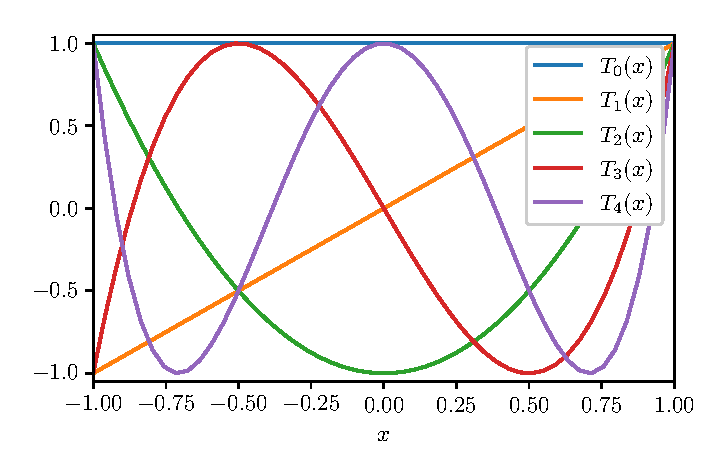
\includegraphics{figures/chebyshevs.eps}
    \caption{Chebyshev polynomials from $ N = 0, \dots, 4 $}
    \label{fig:cheby04}
\end{figure}

% They have the power series \citep{canuto2007spectral}
% \begin{equation}
%     T_k(z) = \frac{k}{2} \sum^{[k/2]}_{l=0} (-1)^k \frac{(k - l - 1)!}{l! (k - 2l)!} (2z)^{k - 2l}.
% \end{equation}

One of the useful properties of Chebyshev polynomials is the fact that we can find recursive relations relating $ T_k(z) $ of different order. Consider the trigonometric identity $ \cos((k + 1) \theta) + \cos((k - 1) \theta) = 2 \cos(\theta) \cos(k \theta) $. If we use $ \theta = \arccos z $ as defined above we end up with the following expression
\begin{gather}
    \cos((k + 1) \arccos z) + \cos((k - 1) \arccos z) = 2 \cos(\arccos z) \cos(k \arccos z).
\end{gather}

Notice that each of the terms of this expression has the form of a different order of Chebyshev polynomial. If we replace each term with its corresponding $ T_k(z) $ and rearrange, we are then left with the following recursion relation
\begin{equation}
    T_{k+1}(z) = 2 z T_k(z) - T_{k-1}(z).
\end{equation}

% This will be extremely useful in Section \ref{section:deriv} when we discuss how to represent the derivatives of a function. 

Before we move on to discussing how we will approximate our function, there is one more useful property of Chebyshev polynomials that we will need. The $k$th order Chebyshev polynomial has $ k $ zeros at the following points \citep{canuto2007spectral}
\begin{equation}
    z_i = \cos(\frac{(1+2i) \pi}{2 k}),\ \ i = 0, \dots, k - 1.
    \label{chebyzeros}
\end{equation}

We will use these in the next section for approximating integrals using the Chebyshev-Gauss quadrature.

% \textbf{gauss quadrature and gauss points from \cite{canuto2007spectral}}

\section{Approximating a function}
We express our function $ \phi $ and its derivatives as a sum of $ M + 1 $ Chebyshev polynomials
\begin{equation}
    \dv[q]{\phi(z)}{z} = \sum^M_{k=0} a_k^{(q)} T_k(z),
    \label{expansion}
\end{equation}
where $ a_k^{(q)} $ are the expansion coefficients of the representation. This function expansion approximates $ \phi $ up to a polynomial of degree $ M $.

We represent our expansion as an $ M + 1 $ dimensional vector $ \mathbf{a} $, where the $k$th component of $ \mathbf{a} $ is the corresponding $ a_k $ from our expansion.
\begin{equation}
    \mathbf{a} = \begin{pmatrix}
        a_0^{(0)} \\
        a_1^{(0)} \\
        \dots \\
        a_{M-1}^{(0)} \\
        a_M^{(0)}
    \end{pmatrix}.
    \label{coeffvec}
\end{equation}

We will now show how to approximate the function
\begin{equation}
    f(z) = \cos(z) = \sum^M_{k=0} a_k T_k(z),
    \label{cos}
\end{equation}
as a sum of Chebyshev polynomials. Note that from now on, $ a_k$ with no superscript will represent $ a_k^{(0)} $, the coefficients corresponding to the expansion of our undifferentiated function.

To calculate our $ a_k $ we multiply both sides of \eqref{cos} by $ T_i(z) / \sqrt{1 - z^2}$ and then integrate between $ -1 $ and $ 1 $. This leaves us with
\begin{align}
    \inte{1}{-1}{\frac{\cos(z) T_i(z)}{\sqrt{1-z^2}}}{z} &= \inte{1}{-1}{\qb{\sum^M_{k=0} a_k T_k(z)} \frac{T_i(z)}{\sqrt{1-z^2}}}{z} \\
    &= \sum^M_{k=0} a_k \inte{1}{-1}{\frac{T_k(z) T_i (z)}{\sqrt{1 - z^2}}}{z}.
    \label{akderiv}
\end{align}

Notice that the integral inside the sum on the right-hand side of \eqref{akderiv} corresponds to the inner product in \eqref{chebyip}. Since Chebyshev polynomials are orthogonal, we are just left with a single coefficient when $ i = k $. This leaves us with
\begin{equation}
    \inte{1}{-1}{\frac{\cos(z) T_i(z)}{\sqrt{1-z^2}}}{z} = a_i c_i \tfrac{\pi}{2},
\end{equation}
which can be rearranged to give us an explicit formula for our $ a_k $ as seen in \citet{canuto2007spectral} 
\begin{equation}
    a_k = \frac{2}{\pi c_k} \inte{1}{-1}{\frac{f(z) T_k(z)}{\sqrt{1-z^2}}}{z}.
\label{coeffexplicit}
\end{equation}
Note: the indices $ i $ and $ k $ have been swapped for consistency with how the coefficients are referenced in our expansion.

We now have a way of calculating the corresponding Chebyshev expansion of $ \cos(z)$. However, before we can implement this in Python we need a method of approximating the integral in \eqref{coeffexplicit}. To do this we will use a Chebyshev-Gauss quadrature method. We can approximate the weighted integral in \eqref{coeffexplicit} as the following sum
\begin{equation}
    \inte{1}{-1}{\frac{g(z)}{\sqrt{1-z^2}}}{z} = \sum^N_{i=0} g(z_i) w_i,
\end{equation}
where the $ z_i $ are the $ N + 1 $ zeros of $ T_{N+1}$ as stated in \eqref{chebyzeros}. It can be shown that the corresponding $ w_i $ are constant with a value of $ \pi / (N+1)$, and that the degree of precision for this approximation is $ 2N + 1 $ \citep{canuto2007spectral}. Substituting this approximation into \eqref{coeffexplicit} leaves us with the following approximation for our $ a_k$
\begin{align}
    a_k &= \frac{2}{\pi c_k} \qb{ \frac{\pi}{N+1} \sum^N_{i=0} f(z_i) \cos(\frac{k (1 + 2i) \pi}{2 (N + 1)})} \\
    &= \frac{2}{c_k (N+1)} \sum^N_{i=0} f(z_i) \cos(\frac{k (1 + 2i) \pi}{2 (N + 1)}). 
\end{align}

We have implemented this method in Python and the code written can be found in Appendix \ref{code:funcapprox}. The approximation for different numbers of polynomials can be found in Figure \ref{fig:cosapprox}. 

\begin{figure}[h!]
    \centering
    \subfloat[Approximation for $ N = 0 $]{
        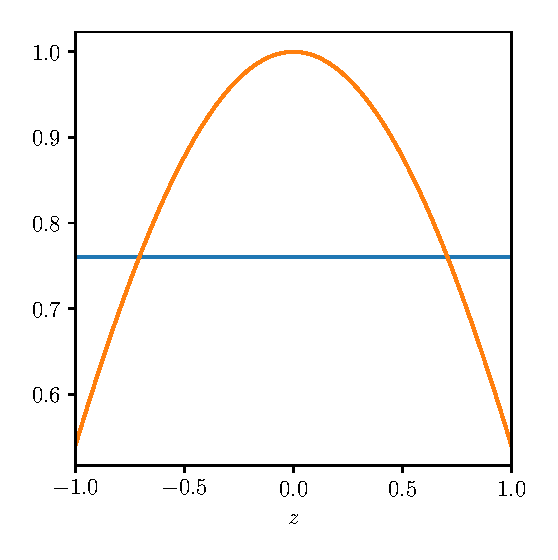
\includegraphics[width=60mm]{figures/cheby_approxN=0.eps}
    }
    \subfloat[Approximation for $ N = 1 $]{
        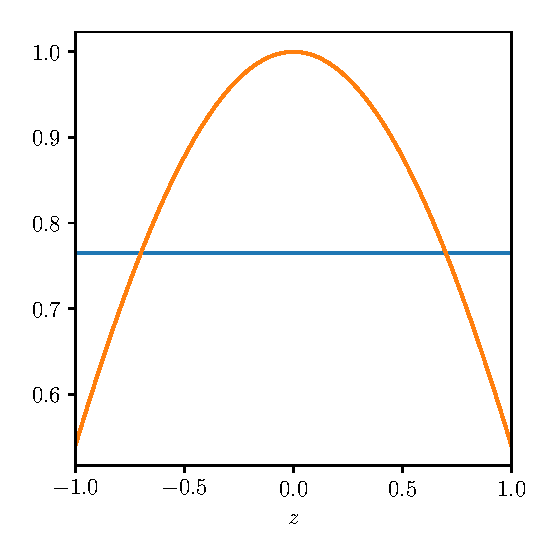
\includegraphics[width=60mm]{figures/cheby_approxN=1.eps}
    }
    \hspace{0mm}
    \subfloat[Approximation for $ N = 2 $]{
        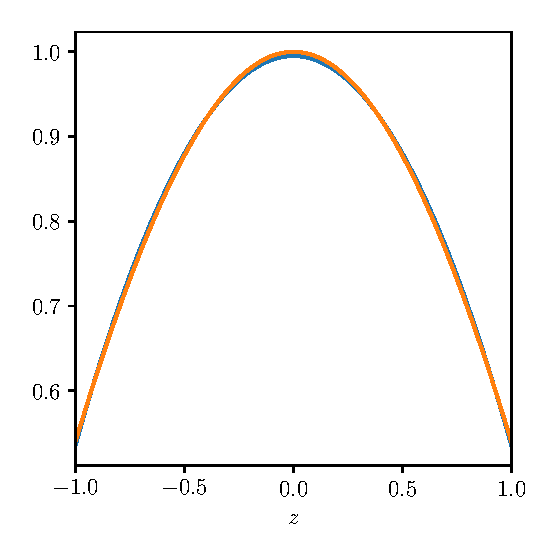
\includegraphics[width=60mm]{figures/cheby_approxN=2.eps}
    }
    \subfloat[Approximation for $ N = 5 $]{
        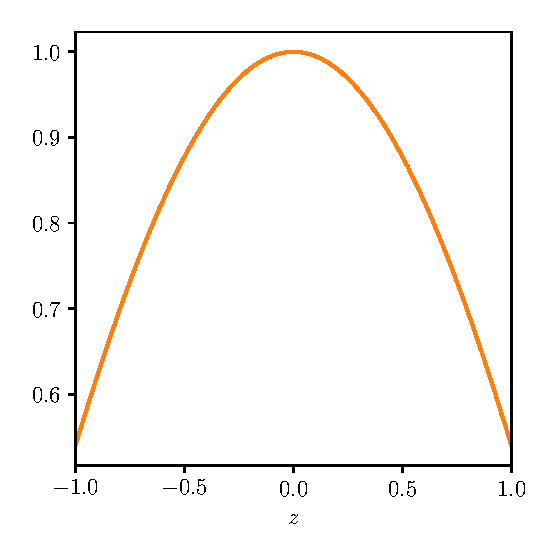
\includegraphics[width=60mm]{figures/cheby_approxN=5.eps}
    }
    \caption{The Chebyshev approximation of $ \cos(z) $ with differing numbers of polynomials (differing values of $ N$). The orange line in each plot corresponds to $ \cos(z)$, while the blue line corresponds to an approximation.}
    \label{fig:cosapprox}
\end{figure}

As can be seen, the approximation doesn't change between $ N = 0 $ and $ N = 1 $. This makes sense as the Taylor expansion of $ \cos z $ around $ z = 0 $ doesn't include any odd powers of $ z$, meaning we wouldn't expect any Chebyshev polynomials with odd order in our approximation. The Chebyshev approximation also clearly converges extremely fast, even with $ N = 2 $ there is very little difference between the approximation and the actual function. Figure \ref{fig:chebyvtaylor} shows a comparison between the second-order Chebyshev approximation of $\cos(z)$ (left), and the second-order Taylor approximation of $ \cos(z)$ (right).  

\begin{figure}[h!]
    \centering
    \subfloat[Second order Chebyshev approximation of $ \cos(z)$]{
        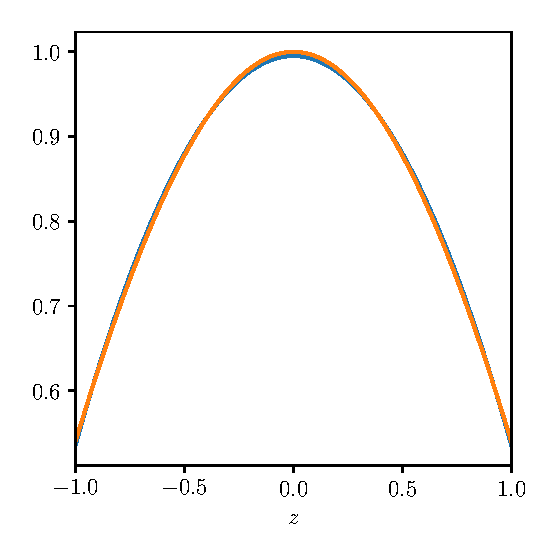
\includegraphics[width=60mm]{figures/cheby_approxN=2.eps}
    }
    \hspace{10mm}
    \subfloat[Second order Taylor approximation of $ \cos(z)$]{
        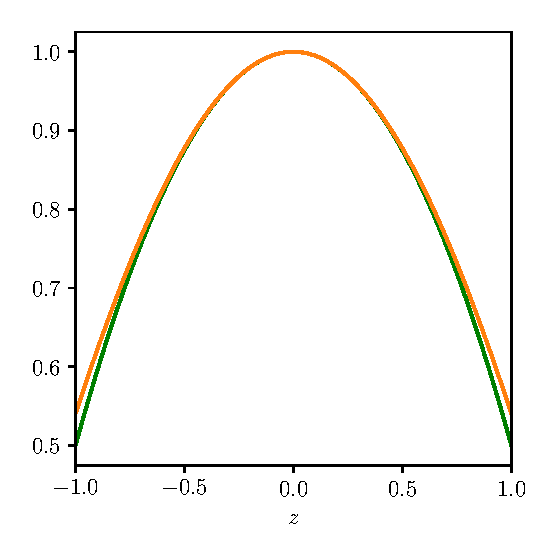
\includegraphics[width=60mm]{figures/taylor_approx.eps}
    }
    \caption{The Chebyshev approximation of $ \cos(z) $ with $ N = 2 $ blue line compared to the Taylor approximation of $ \cos(z) $ (green line).}
    \label{fig:chebyvtaylor}
\end{figure}

We can see that while the Chebyshev approximation takes an incorrect value at $ z = 0 $, there is a significant divergence between the Taylor approximation and $ \cos(z) $ at the endpoints. This implies that the Chebyshev approximation converges to $ \cos(z)$ much faster than the Taylor approximation.

Now we have a method of approximating a function, we need a method of representing the derivatives of a function in terms of some matrix $ D^m $ multiplied by our approximation vector $ \mathbf{a} $, where $m $ represents the order of derivative we are calculating. This will allow us to represent the action of differential operators on our expansion as the action of a matrix on our expansion. Calculating the form of $ D^m$ is the focus of the next section.

\section{Representing derivatives} \label{section:deriv}

Differentiating \eqref{cheby} with respect to $ z $ implies that the first derivative of the $k$-th order Chebyshev polynomial has the following form
\begin{equation}
    \dv{z} T_k(z) = \frac{-k \sin(k \arccos z)}{\sqrt{1 - z^2}} = \frac{-k \sin(k \theta)}{\sin \theta}, 
\label{chebyderiv}
\end{equation}
where $ z = \cos \theta $ as before. 

There are $ 2 $ important things to note from this definition:
\begin{enumerate}
    \item We have that $ T_k'(z) = T_{-k}'(z) $.
    \item We have the limit $ \lim_{k \rightarrow 0} T_k'(z) / k = \lim_{k \rightarrow 0} -\sin(k \theta) / \sin \theta = 0 $.
    \label{divprops}
\end{enumerate}

If  now we consider the trigonometric relation $ 2 \sin \theta \cos \theta = \sin(k+1)\theta - \sin(k-1)\theta $ we have that 
\begin{align}
    2 \cos \theta &= \frac{\sin((k+1) \theta)}{\sin \theta} - \frac{\sin((k-1) \theta)}{\sin \theta}, \\
    2 T_k(z) &= \frac{1}{k+1} T'_{k+1}(z) - \frac{1}{k-1}T'_{k-1}(z),
    \label{chebrelation}
\end{align}
which gives us a recursive relation between different orders of derivatives of Chebyshev polynomials. 

We would like to use this recursion relation to find a recursion relation between the coefficients of our undifferentiated function $ a_k$ and the coefficients of a derivative of our function $ a_k^{(q)} $. If we consider the first derivative of a perfect expansion of the form in \eqref{expansion} (i.e. the case where $ N = \infty $, we can see that the following are equivalent
\begin{equation}
    \sum^\infty_{k=0} a^{(0)}_k T_k' (z) = \dv{\p}{z} = \sum^\infty_{k = 0} a_k^{(1)} T_k.
\end{equation}

We can use this result along with the recursion relation \eqref{chebrelation} to get the following
\begin{align}
    \sum^\infty_{k=0} a_k^{(0)} T_k'(z) &= \tfrac{1}{2} \sum^\infty_{k=0} a_k^{(1)} \qb{\frac{1}{k+1} T_{k+1}'(z) - \frac{1}{k - 1} T_{k-1}'(z)} \\ 
    &= \tfrac{1}{2} \qb{\sum^\infty_{k=0} \frac{a_k^{(1)}}{k+1} T_{k+1}'(z) - \sum^\infty_{k=0} \frac{a_k^{(1)}}{k-1} T_{k-1}(z)}. \label{divsums}
\end{align}

To get a recursion relation between our coefficients, we would like to be able to compare the terms of the sums in \eqref{divsums}. Define $ n = k + 1 $ and $ m = k - 1$. If we use these as the indices in the two sums on the right of \eqref{divsums} we get the following
\begin{align}
    \sum^\infty_{k=0} a_k^{(0)} T_k'(z) &= \tfrac{1}{2} \qb{\sum^\infty_{n=1} \frac{a_{n-1}^{(1)}}{n} T_n'(z) - \sum^\infty_{m=-1} \frac{a_{m+1}^{(1)}}{m} T_m'(z)} \\
    &= \tfrac{1}{2} \qb{\sum^\infty_{k=1} \qb{\frac{a_{k-1}^{(1)}}{k} - \frac{a_{k+1}^{(1)}}{k}} T_k'(z) + a_0^{(1)} T_{-1}'(z) - \frac{a_1^{(1)}}{0} T_0(z)}. 
\end{align} 
Notice that $ T_1'(z) = T_{-1}'(z) $ in the second to last term thanks to the first of the properties of the derivative \eqref{chebyderiv} and that the last term vanishes thanks to the second of the properties of the derivative \eqref{chebyderiv}. This leaves us with
\begin{align}
    \sum^\infty_{k=0} a_k^{(0)} T_k'(z) &= \tfrac{1}{2} \sum^\infty_{k=1} \qb{\frac{c_{k-1} a_{k-1}^{(1)}}{k} - \frac{a_{k+1}^{(1)}}{k} T_k'(z)},
\intertext{From here we extract our recursion relation for our coefficients}
    2 k a_k^{(0)} &= c_{k-1} a_{k-1}^{(1)} - a_{k+1}^{(1)},\ \ k \geq 1. \label{coeffrelation}
\end{align}

We would like an expression for $ a_k^{1} $ that only uses $ a_p $ for various $p \geq 0 $. If we apply \eqref{coeffrelation} to itself we get 
\begin{align}
    c_{k - 1} a_{k-1}^{(1)} &= 2 k a_k + a_{k+1}^{(1)} \\
    &= 2k a_k + (2(k+2) a_{k+2} + a_{k+3}^{(1)} \\
    &= 2k a_k + 2(k+2) a_{k+2} + (2(k+4) a_{k + 4} + a_{k+5}^{(1)}) \\
    & \ \ \vdots
\end{align}

If we continue this process up to a truncation point of $ M $ polynomials, we obtain the following formula for the coefficients of the first derivative of $ \phi $ as seen in the literature \citep{canuto2007spectral, orszag1971accurate} 
\begin{equation}
    a_k^{(1)} = \frac{2}{c_k} \sum^{M}_{\substack{p = k + 1 \\ p \equiv 1\ (\text{mod } 2)}} p a_p. \label{divsum}
\end{equation}

To get higher derivatives we can just apply this method recursively. The second derivative is obtained by the following 
\begin{equation}
    a_k^{(2)} = \frac{2}{c_k} \sum^{M}_{\substack{p = k + 1 \\ p \equiv 1\ (\text{mod } 2)}} p a_p^{(1)}.
\end{equation}

Applying the sum \eqref{divsum} again, we can get an expression for the coefficients of the $2$nd derivative of $ \phi$ given by
\begin{equation}
    a^{(2)}_{k} = \frac{1}{c_k} \sum^{M}_{\substack{p = k + 2 \\ p \equiv 0\ (\text{mod } 2)}} p (p^2 - k^2) a_p.
\end{equation}

In a similar way, we can compute an expression for $ a^{(4)}_k $ given by
\begin{equation}
    a^{(4)}_k = \frac{1}{c_k} \sum^N_{\substack{p = k + 4 \\ p \equiv 0\ (\text{mod } 2)}} p [p^2 (p^2 - 4)^2 - 3 k^2 p^4 + 3 k^4 p^2 - k^2 (k^2 - 4)^2] a_k.
    \label{d4expansion}
\end{equation}

It is clear that for large $ p $ and $ k $, \eqref{d4expansion} grows extremely fast. This means that numerically we can lose significance as $ M $ becomes large. To reduce this, \cite{herbert1977neutrale} suggested that the substitution $ q = p - k $ be used inside the brackets. This transforms \eqref{d4expansion} into
\begin{equation}
    a^{(4)}_k = \frac{1}{c_k} \sum^N_{\substack{p = k + 4 \\ p \equiv 0\ (\text{mod } 2)}} p [q^4 (q^2 - 8) + k q^3 (6 q^2 - 32) + (12 k^2 q^2 + 8 k^3 q)(q^2 - 4) + 16 q^2 + 32 kq] a_k.
    \label{qd4expansion}
\end{equation}

We can then represent the coefficients of a derivative of $ \p $ by multiplying our vector $ \mathbf{a} $ by an $ (M + 1) \cross (M + 1) $ matrix $ D^n $

For $ n = 1 $, we have
\begin{equation}
D = \begin{pmatrix}
    0 & 1 & 0 & 3 & 0 & 5 & 0 & 7 & 0 & \dots\\
    0 & 0 & 4 & 0 & 8 & 0 & 12 & 0 & 16 & \dots\\
    0 & 0 & 0 & 6 & 0 & 10 & 0 & 14 & 0 & \dots\\
    0 & 0 & 0 & 0 & 8 & 0 & 12 & 0 & 16 & \dots\\
    0 & 0 & 0 & 0 & 0 & 10 & 0 & 14 & 0 & \dots\\
    0 & 0 & 0 & 0 & 0 & 0 & 12 & 0 & 16 & \dots\\
    \ds & \ds & \ds & \ds & \ds & \ds & \ds & \ds & \ds & \ds 
\end{pmatrix}.
\label{D}
\end{equation}

For $ n = 2 $, we have
\begin{equation}
D^2 = \begin{pmatrix}
    0 & 0 & 4 & 0 & 32 & 0 & 108 & 0 & 256 & \dots\\
    0 & 0 & 0 & 24 & 0 & 120 & 0 & 336 & 0 & \dots \\
    0 & 0 & 0 & 0 & 48 & 0 & 192 & 0 & 480 & \dots \\
    0 & 0 & 0 & 0 & 0 & 80 & 0 & 280 & 0 & \ds\\
    0 & 0 & 0 & 0 & 0 & 0 & 120 & 0 & 384 & \ds\\
    0 & 0 & 0 & 0 & 0 & 0 & 0 & 168 & 0 & \ds\\
    \dots & \dots & \dots & \dots & \dots & \dots & \dots & \dots & \ds & \ds
\end{pmatrix}.
\label{D2}
\end{equation}

For $ n = 4 $, we have
\begin{equation}
    D^4 = \begin{pmatrix}
        0 & 0 & 0 & 0 & 192 & 0 & 4608 & 0 & 38400 & \ds\\
        0 & 0 & 0 & 0 & 0 & 1920 & 0 & 26880 & 0 & \ds\\
        0 & 0 & 0 & 0 & 0 & 0 & 5760 & 0 & 61440 & \ds\\
        0 & 0 & 0 & 0 & 0 & 0 & 0 & 13440 & 0 & \ds\\
        0 & 0 & 0 & 0 & 0 & 0 & 0 & 0 & 26880 & \ds\\
        0 & 0 & 0 & 0 & 0 & 0 & 0 & 0 & 0 & \ds\\
        \ds & \ds & \ds & \ds & \ds & \ds & \ds & \ds & \ds & \ds
    \end{pmatrix}.
    \label{D4}
\end{equation}

Notice that $ D^2 $ and $ D^4 $ are in fact multiples of $ D $. This means in theory we can get any derivative of $ \p $ we want. 

These matrices are implemented in Python in the code in Appendix \ref{code:tau_matrices}. We can then test them by multiplying the coefficients of our computed approximation for $ \cos(z) $ by the matrices $ D, D^2, D^4$ to get the coefficients of the expansion of our derivatives. Note that since $ D^4$ is all zeroes if $ N \leq 4 $ we need to compute an approximation to $ \cos(z) $ that is of a higher order than order $ 4 $. Figure \ref{fig:cosderivapprox} shows the original approximation for $ N = 8 $, along with the approximation for the first, second and fourth derivatives of $ \cos(z)$.

\begin{figure}[h!]
    \centering
    \subfloat[Base approximation to $ \cos(z)$]{
        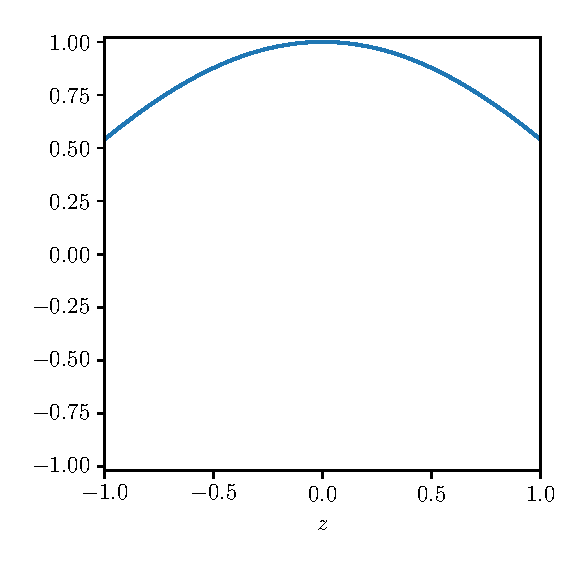
\includegraphics[width=60mm]{figures/chebyapprox_order=8.eps}
    }
    \subfloat[First derivative approximation]{
        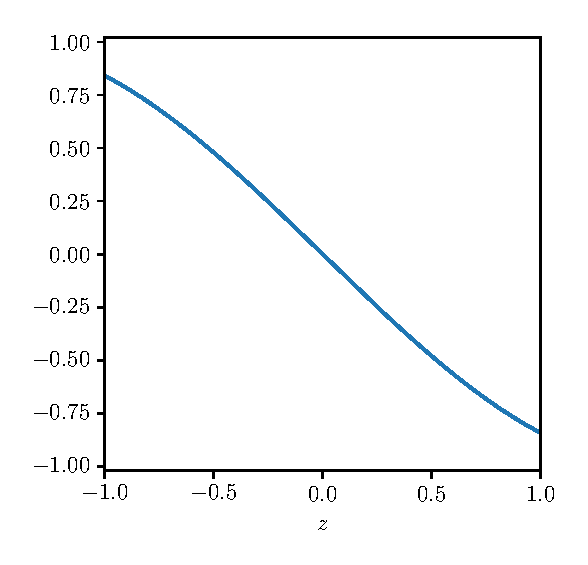
\includegraphics[width=60mm]{figures/diff1approx_order=8.eps}
    }
    \hspace{0mm}
    \subfloat[Second derivative approximation]{
        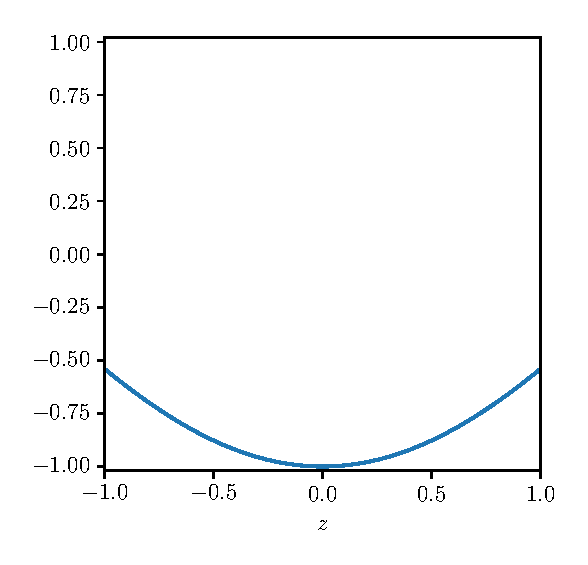
\includegraphics[width=60mm]{figures/diff2approx_order=8.eps}
    }
    \subfloat[Fourth derivative approximation]{
        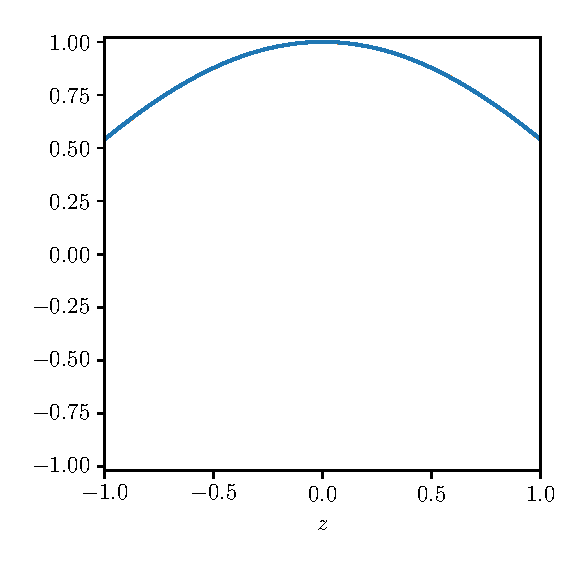
\includegraphics[width=60mm]{figures/diff4approx_order=8.eps}
    }
    \caption{The Chebyshev approximation of $ \cos(z) $ for $ N = 8 $, compared with the Chebyshev approximations of its derivatives. The (obscured) orange line in each plot corresponds to an exact derivative of $ \cos(z)$, while the blue line corresponds to the Chebyshev approximation of that derivative.}
    \label{fig:cosderivapprox}
\end{figure}

From this, we can see that this method for calculating a derivative approximation is extremely accurate. This will allow us to represent differential operators as the action of a matrix on our vector $ \mathbf{a}$. For example, the matrix $ L $ representing the action of the differential operator
\begin{equation}
    \mathcal{L} = \dv[4]{z} + 4 \dv[2]{z} - \dv[1]{z},
\end{equation} 
would have the form
\begin{equation}
    L = D^4 + 4 D^2 - D.
\end{equation}

We can now move on to discussing how we can apply these to represent the Orr-Sommerfeld equation in terms of these matrices.

\section{Fourth Order System}
To get the eigenvalues of the Orr-Sommerfeld equation we would like a generalised eigenvalue problem of the form 
\begin{equation}
    A \mathbf{a} = c B \mathbf{a},
\end{equation}
where $\mathbf{a}$ is the $ M + 1$ dimensional vector representing the coefficients of the Chebyshev expansion of our eigenfunction $ \phi$, and $ A $ and $B $ are $ (M + 1) \cross (M + 1) $ matrices.

To get matrix expressions for $A $ and $B $ we rearrange the Orr-Sommerfeld equation \eqref{oseq} to be in the following form
\begin{equation}
    (i \al R)^{-1} (D^4 - 2 \al^2 D^2 + \al^4) \p - U (D^2 - \al^2) \p + U'' \p = -c (D^2 - \al^2) \p. 
    \label{osrearrange}
\end{equation}

From here we can see that $ A $ and $ B $ take the following forms
\begin{align}
    A &= (i \al R)^{-1} (D^4 - 2 \al^2 D^2 + \al^4 I) - U (D^2 - \al^2 I) + U'' I, \\
    B &= -(D^2 - \al^2 I).
\end{align}

How do we represent our $ U $ and $ U'' $? The best way to do this is to work out some matrix that we can then multiply our coefficients for the expansion of $ \p$ and $ D^2 \p$ by \citep{bukhari1997spectral}. To do this let us assume we can accurately compute a Chebyshev expansion for our $ U $ and $ U''$ of the form
\begin{equation}
    u(z) = \sum^\infty_{j=0} b_j T_j(z).
\end{equation}

We then would like to consider the product 
\begin{align}
    h(z) &= u(z) \p(z) \\
    &= \sum^\infty_{j=0} \sum^M_{k=0} a_k b_j T_j(z) T_k(z),
    \label{chebyprod}
\end{align}
of $ 2 $ Chebyshev expansions. Can we represent the product $ T_j(z) T_k(z) $ in a nicer way? If we consider the trigonometric relation
\begin{equation}
    \cos(i \theta) \cos(j \theta) = \frac{\cos((i + j)\theta) + \cos((i - j) \theta) }{2},
\end{equation}
with $ \theta = \arccos(z)$ then we end up with the following
\begin{align}
    T_i(z) T_j(z) &= \frac{T_{i+j}(z) + T_{i-j}(z) }{2} \\
    &= \frac{T_{i+j}(z) + T_{\abs{i-j}}(z)}{2},
\end{align}
where the $ \abs{i-j}$ just comes from the fact that $ T_k(z) = T_{-k}(z) $. If we substitute this back into the product \eqref{chebyprod} we get the following
\begin{align}
    h(z) &=  \tfrac{1}{2} \sum^\infty_{j=0} \sum^M_{k = 0} a_k b_j \qb{T_{j + k}(z) + T_{\abs{j - k}}(z)} \\
    &= \tfrac{1}{2} \sum^\infty_{j=0} \sum^M_{k = 0} a_k b_j T_{j + k}(z) + \tfrac{1}{2} \sum^\infty_{j=0} \sum^M_{k = 0} a_k b_j T_{\abs{j - k}}(z).
    \label{hz}
\end{align}

If we change indices to $ n = j + k$ in the first sum, we can split the first sum into two separate sums. We have that $ b_{n - k} = 0 $ if $ n - k < 0$. This implies that if $ n < M$, we only have non-zero $ b_{n - k}$ if $ k \leq n $. If $ n > M$ we have that $ k \leq M $. This means that the following holds
\begin{equation}
    \tfrac{1}{2} \sum^\infty_{j=0} \sum^M_{k = 0} a_k b_j T_{j + k}(z) = \tfrac{1}{2} \sum^{M}_{n=0} \sum^n_{k=0} a_k b_{n - k} \T{n} + \tfrac{1}{2} \sum^\infty_{n=M} \sum^M_{k=0} a_k b_{n -k} \T{n}.
\end{equation}

For the second sum, there are two cases to consider. If $ j \leq k$ , $ \T{\abs{j - k }} = \T{k - j}$. If we substitute $ m = k - j $ then we end up with that $ m $ must take a range of between $ 0 $ and $ M$ and that $ k $ must be larger than $ m$, meaning we have the sum 
\begin{equation}
    \sum^M_{m=0} \sum^M_{k=m} a_k b_{k - m} \T{m}.
\end{equation}
If $ j > k $, if we let $ p = j - k$ we end up with the final sum 
\begin{equation}
    \sum^\infty_{p=1} \sum^M_{k=0} a_k b_{p+k} \T{p}.
\end{equation}
Notice that $ p $ starts at $ 1 $ rather than $ 0$. This is because we already have the product $ a_0 b_0 $ in the first of these two sums.

Substituting these results back into \eqref{hz} gives us our product split into $ 4 $ sums (as seen in \citet{bukhari1997spectral})
\begin{align}
    h(z) &= \tfrac{1}{2} \sum^{M}_{n=0} \sum^n_{k=0} a_k b_{n - k} \T{n} + \tfrac{1}{2} \sum^\infty_{n=M} \sum^M_{k=0} a_k b_{n -k} \T{n} \\ &+ \tfrac{1}{2} \sum^M_{n=0} \sum^M_{k=n} a_k b_{k - n} \T{n} + \tfrac{1}{2} \sum^\infty_{n=1} \sum^M_{k=0} a_k b_{n+k} \T{p},
\end{align}
where we have made the indices the same for clarity.

We can represent this product as an $ (M+1) \cross (M+1) $ matrix multiplied by a vector of the $ M + 1 $ coefficients of our function $ \p(z)$. This means each element of the matrix $ A_{nk} $ will correspond to the sum of the $ b_n $ that are multiplied by $ a_k$. For example, for $ n = 0$, we have that the first row would represent the sum
\begin{equation}
    a_0 b_0 + \tfrac{1}{2} \sum^M_{n = 1} a_n b_n,
\end{equation}
and would therefore have the row vector form
\begin{equation}
    \tfrac{1}{2} \begin{pmatrix}
        2b_0 & b_1 & b_2 & \dots & b_{M}
    \end{pmatrix}.
\end{equation}

From here on, we will represent the matrices for $ U'' $ and $ U$ by $ P $ and $ Q $ respectively as in \citet{bukhari1997spectral}.

%There are a number of methods for this. 
%In \cite{orszag1971accurate} he explicitly calculates the case for plane Poiseuille flow and therefore only has to deal with the $ z^2 $ term. Orszag computes a sum for the $k$th coefficient of $ z^2 \phi^{(n)}$ which has the following form 
% \begin{equation}
%     \tfrac{1}{4} (c_{k-2} a_{k -2}^{(n)} + (c_k + c_{k-1}) a_k^{(n)} + a_{k+2}^{(n)}).
% \end{equation}

% We can translate this into a matrix 
% \begin{equation}
%     C = \begin{pmatrix}
%         0.5 & 0 & 0.25 & 0 & 0 & 0 & 0 & \ds \\
%         0 & 0.75 & 0 & 0.25 & 0 & 0 & 0 & \ds \\
%         0.5 & 0 & 0.5 & 0 & 0.25 & 0 & 0 & \ds \\
%         0 & 0.25 & 0 & 0.5 & 0 & 0.25 & 0 & \ds \\
%         \ds & \ds & \ds & \ds & \ds & \ds & \ds & \ds
%     \end{pmatrix}.
% \end{equation}

% We can then get $ z^2 D^2 \p $ by multiplying $ D^2 \mathbf{a} $ by $ C $. Our $  U (D^2 - \al^2 I)$ then becomes $ (I - C)(D^2 - \al^2 I) $ for plane Poiseuille flow. 

% Another method is as in \cite{bukhari1997spectral} where we use matrices $ P $ and $ Q $ to represent the $ U'' $ and $ U $ terms respectively. 

For plane Poiseuille flow we have that $ U'' = -2 = -2 \T{0} $ which means that we just have that $ b_0 = -2 $ for its expansion and $ U = 1 - z^2 = \tfrac{1}{2} \T{0} - \tfrac{1}{2} \T{2} $, meaning that for the expansion of $ U $ we have that $ b_0 = \tfrac{1}{2}$ and $ b_2 = -\tfrac{1}{2} $. This means we have the following forms for $ P $ and $ Q $
\begin{equation}
    P = -2 I,\ \ Q = \begin{pmatrix}
        0.5 & 0 & -0.25 & 0 & \dots \\
        0 & 0.25 & 0 & -0.25 & \dots \\
        -0.5 & 0 & 0.5 & 0 & \dots \\
        0 & -0.25 & 0 & 0.5 & \dots \\
        \dots & \dots & \dots & \dots & \dots
    \end{pmatrix}.
\end{equation}

For Couette flow $ U'' = 0 $ and $U = z = \T{1} $, implying that $P $ and $ Q $ have the following forms
\begin{equation}
    P = 0,\ Q = \begin{pmatrix}
        0 & 0.5 & 0 & 0 & \ds \\
        1 & 0 & 0.5 & 0 & \ds \\
        0 & 0.5 & 0 & 0.5 & \ds \\
        0 & 0 & 0.5 & 0 & \ds \\
        \ds & \ds & \ds & \ds & \ds
    \end{pmatrix}.
\end{equation}

Note: When $ P $ and $ Q $ are given in \cite{bukhari1997spectral} for the case of Poiseuille flow, $ P $ is mistakenly stated to be $ 2 I $ instead of $ -2 I$ as here. 

If we use the $ P $ and $ Q $ matrices, we end up with these final forms for matrices $ A $ and $B$
\begin{align}
    A &= (i \al R)^{-1} (D^4 - 2 \al^2 D^2 + \al^4 I) - Q (D^2 - \al^2 I) + P, \\
    B &= -(D^2 - \al^2 I).
    \label{4thblockform}
\end{align}

We now have a generalised eigenvalue problem of the form $ A \mathbf{a} = c B \mathbf{a} $ which can be solved in Python. Details of exactly how this will be done are given in \ref{section:solving}.

Notice that the terms of our $ D^4 $ matrix \eqref{D4} scale with $ O(M^7) $ and the terms of our $ D^2 $ matrix \eqref{D2} scale with $ O(M^3) $. This means it is better to only use the lower-order differentiation matrices if possible. The next section will explore how to do this in the $2$nd order case. 

\section{Second Order System}
How do we make our system require only the use of $D^2$? The answer is to split the Orr-Sommerfeld equation into a system of $2$nd order equations. We define $ \phi_1 = \phi,\ \phi_2 = D^2 \phi $. These two functions allow us to represent the Orr-Sommerfeld equation \eqref{oseq} as the following system of $2$nd order differential equations
\begin{align}
    \phi_2 &= D^2 \phi_1, \\
    (i \alpha R)^{-1} ((D^2 - 2 \alpha^2) \phi_2 + \alpha^4 \phi_1) &= (U - c)(\phi_2 - \alpha^2 \phi_1) - U'' \phi_1.
    \label{2ndorder}
\end{align}

Rearrange these to get
\begin{subequations}
\begin{align}
    D^2 \phi_1 - \phi_2 &= 0, \label{2ndeq1} \\
    (U \al^2 + U'') \phi_1 + ((i \al R)^{-1} ((D^2 - 2 \al^2) - U) \phi_2 + \al^4 \phi_1) &= c \al^2 \phi_1- c\phi_2. \label{2ndeq2}
\end{align}
\end{subequations}

We want to put these into a generalised eigenvalue problem of the form $ E \mathbf{b} = c F \mathbf{b} $ like for the $4$th order case.

To begin let us work out what our vector $ \mathbf{b} $ is. If we denote the vector associated to our expansion of $ \phi_1 $ by $\mathbf{a}_1$ and the vector associated to our expansion of $ \phi_2 $ by $ \mathbf{a}_2 $ then we can form $ \mathbf{b} = (\mathbf{a}_1, \mathbf{a}_2)^\intercal $. This vector is $ 2(M+1) $ dimensional so therefore our matrices are $ 2(M+1) \cross 2(M+1) $ matrices. 

We set $E$ and $F$ out as in \cite{bukhari1997spectral}, with the first $ M + 1 $ rows corresponding to equation \eqref{2ndeq1} and the last $ M + 1 $ rows corresponding to equation \eqref{2ndeq2}. The first $ M + 1$ columns will correspond to operations done to $ \phi_1$ and the last $ M + 1 $ columns will correspond to operations done to $\phi_2$. This leaves us with the following forms for $E$ and $F$,
\begin{equation}
    E = \begin{pmatrix}
        D^2 & -I \\
        (P - \alpha^2 Q) + (i R)^{-1} \alpha^3 I & (i \alpha R)^{-1} (D^2 - 2 \alpha^2 I) - Q
    \end{pmatrix},\ \
    F = \begin{pmatrix}
        0 & 0 \\
        \alpha^2 I & -I
    \end{pmatrix}.
\label{2ndblockform}
\end{equation}

This leaves us with a generalised eigenvalue problem of the form $ E \mathbf{b} = c B \mathbf{b} $, which we can solve in the same way as our $4$th order system. Solving this should yield significantly lower numerical error than our $4$th order system. However, we can reduce the numerical error further by splitting \eqref{2ndorder} further into a system of $1$st order differential equations.

\section{First Order System}

To create a system where we only use $ D$ we need to split the Orr-Sommerfeld equation \eqref{oseq} into a system of $1$st order differential equations. To do this we define
\begin{equation} \phi_1 = \phi,\ \phi_2 = D \phi,\ \phi_3 = D^2 \phi, \phi_4 = D^3 \phi.
\label{p4}
\end{equation}

From here we have the following system of $1$st order equations
\begin{subequations}
    \begin{align}
        D \phi_1 &= \phi_2, \\
        D \phi_2 &= \phi_3, \\
        D \phi_3 &= \phi_4, \\
        (i \al R)^{-1} \phi_4 &= (i \al R)^{-1} (2 \al^2 \phi_3 - \al^4 \p_1) + (U - c)(\phi_3 - \al^2 \phi_1) - U'' \p_1.
    \end{align}
    \label{1storder}
\end{subequations}

Again we want these in the form $ G \mathbf{c} = c H \mathbf{c} $, so we rearrange the equations of \eqref{1storder} to get 
\begin{subequations}
\begin{align}
    D \p_1 - \p_2 &= 0, \\
    D \p_2 - \p_3 &= 0, \\
    D \p_3 - \p_4 &= 0, \\
    (i \al R)^{-1} D \phi_4 - (i \al R)^{-1} (2 \al^2 - U) \phi_3 + ((i \al R)^{-1} \al^4 + U \al^2  + U'') \phi_1 &= - c \phi_3 + c \al^2 \phi_1.
\end{align}
\label{1stordereq}
\end{subequations}

In the same way as the second order case, we represent the vectors corresponding to the expansions of our $4$ functions $ \p_i$ by $\mathbf{a_i} $ with $ i = 1, \dots, 4 $. We set $ \mathbf{c} = (\mathbf{a}_1, \mathbf{a}_2, \mathbf{a}_3, \mathbf{a}_4)^\intercal $. We now have a $ 4(M+1)$ dimensional vector $ \mathbf{c}$ which means that $G$ and $H$ will be $ 4(M+1) \cross 4(M+1) $ matrices.

We again follow the layout of $ G $ and $H$ as in \cite{bukhari1997spectral}. Column $ (i-1)(M+1) $ to column $ i (M+1) $ correspond to the expansion coefficients of $ \p_i $ for $ i = 1, \dots, 4$. Likewise, the rows of $G$ and $H$ are filled by the matrices corresponding to equations \eqref{1stordereq} in groups of $ M+ 1$ rows.

This leaves us with the following forms for $G$ and $H$,
\begin{equation}
    G = \begin{pmatrix}
        D & -I & 0 & 0 \\
        0 & D & -I & 0 \\
        0 & 0 & D & -I \\
        (P + \al^2 Q) + (i R)^{-1} \al^3 & 0 & -Q - (i R)^{-1} (2 \al^2) I &   (i \al R)^{-1} D
    \end{pmatrix},\ \ 
    H = \begin{pmatrix}
        0 & 0 & 0 & 0 \\
        0 & 0 & 0 & 0 \\
        0 & 0 & 0 & 0 \\
        \al^2 I & 0 & -I & 0
    \end{pmatrix}.
\label{1stblockorder}
\end{equation}

We now have a generalised eigenvalue problem $ G \mathbf{c} = c H \mathbf{c} $ that we can again solve. This system has lower numerical error than both of the other methods we have discussed but takes much longer due to the massively increased size of the matrices involved even compared to the second-order method.

\section{Boundary Conditions} \label{section:bc}
Before we can solve the resulting systems from any of our methods, we need a way to represent our boundary conditions. The Orr-Sommerfeld equation has the following boundary conditions, 
\begin{equation}
    \p(\pm 1) = \p'(\pm 1) = 0.
\end{equation}

By using the two properties \eqref{chebyprop} we get the following equations for these boundary conditions
\begin{align}
    \p(1) &=\sum^M_{k=0} a_k, \\
    \p(-1) &= \sum^M_{k=0} (-1)^k a_k, \\
    \p'(1) &= \sum^M_{k=0} k^2 a_k, \\
    \p'(-1) &= \sum^M_{k=0} (-1)^k k^2 a_k = 0.
    \label{bcsums}
\end{align}

If we combine our matrices for any of our methods with these equations we have $ M + 5 $ equations for $ M + 1 $ unknowns, meaning that our system is over-determined and only has the trivial solution $ a_k = 0 $. To solve this we follow the method that \cite{orszag1971accurate} used, to do this we $ 4 $ of the rows of our matrices with boundary equations so that we have $ M + 1 $ equations in $ M + 1 $ unknowns.

For the $4$th order system, we simply replace the last $4$ rows of $ A $ and $B$ in \eqref{4thblockform} with row vectors representing our boundary conditions in $A$ and a row of zeroes in $B$.

We follow a similar procedure for the $2$nd order case. In this case, all $4$ boundary conditions are applied to $\phi_1$ and none to $ \phi_2 $. This is because $\phi_2 = D^2 \phi $. This means the rows inserted into matrix $E$ of \eqref{2ndblockform} will be of the form $ (\mathbf{v}, \mathbf{0})$ where $ \mathbf{v}$ is the $ M+1 $ dimensional vector representing one of the $4$ sums given in \eqref{bcsums} and $\mathbf{0} $ is the $ M +1 $ dimensional zero vector. 

We replace the $ (M - 1)th,\ Mth,\ 2(M-1)th \text{ and } 2Mth$ rows of $E$ and $F$. As with the $4$th order case, the rows replaced in $F$ are just replaced with rows of zeroes. The specific order of how the rows are inserted does not matter \citep{bukhari1997spectral}.

Finally, we deal with the $1$st order system. In this case, we apply the first two boundary conditions to $ \phi_1 $ and the first two boundary conditions again to $ \phi_2$. This is because $ \phi_2 $ represents the first derivative of $ \phi $ and therefore we don't need to apply the boundary conditions that fix the derivative of a function. 

The rows representing the boundary conditions applied to $\phi_1$ have the form $ (\mathbf{v}, \mathbf{0}, \mathbf{0}, \mathbf{0}) $ and the rows representing the boundary conditions applied to $ \phi_2 $ have the form $ (\mathbf{0}, \mathbf{v}, \mathbf{0}, \mathbf{0}) $. They are inserted into the $Mth,\ 2Mth,\ 3Mth\ \text{and}\ 4Mth$ rows of $ G $ and $H$. Again we insert just rows of zeroes into $H$.

We now can move on to solving our systems.

\section{Solving our system} \label{section:solving}
For each of the above methods we now have a generalised eigenvalue problem of the form
\begin{equation}
    A \mathbf{b} = c B \mathbf{b}.
    \label{geneigproblem}
\end{equation}
We implement this system in Python (the code for this is found in the appendix), but we have a problem! The matrix $ B $ is singular due to the rows of zeros added by the boundary conditions, which means we cannot rearrange \eqref{geneigproblem} to be in the form $ A B^{-1} \mathbf{b} = c \mathbf{b} $ and therefore cannot be solved using just any eigenvalue method. 

To solve them we use the QZ algorithm of \cite{moler1973algorithm}, as suggested by \cite{dongarra1996chebyshev} which allows us to get the eigenvalues of this problem even though the matrix $ B $ is singular. In Python, this is implemented in the \codeword{scipy.linalg.eig} function in the \codeword{scipy} package, a link to which is found \href{https://docs.scipy.org/doc/scipy/reference/generated/scipy.linalg.eig.html}{\textcolor{blue}{here}}. 

The reason that the QZ algorithm is preferred is two-fold. Firstly, the QZ algorithm can find all of the eigenvalues of the system \eqref{geneigproblem} and does not require knowledge of the position of the eigenvalues as with shooting or search methods. This is useful for this case as we are searching for any eigenvalue with an imaginary part above $0$ and therefore want all possible eigenvalues of our system. Secondly, as shown in \cite{dongarra1996chebyshev}, using a search technique such as \cite{orszag1971accurate} can 'miss out' eigenvalues. 

The QZ algorithm transforms $A $ and $B$ using Householder transformations and then calculates their eigenvalues as $ \al_i$ and $ \beta_i$, where the $ \al_i$ are the eigenvalues of $A $ and the $ \beta_i$ are the eigenvalues of $ B$. The eigenvalues of our system are then obtained by dividing each $ \al_i$ by its respective $ \beta_i$. As our system is singular, we would expect some of our eigenvalues to be 'infinite' or 'spurious' eigenvalues caused by this singularity. An additional advantage of the QZ algorithm is that we can filter out these 'spurious' eigenvalues by checking the $ \beta_i$. Specifically, we remove any that are zero.

We now have several numerical methods implemented that can be used to assess the stability of flows for various values of $ R $. The focus of the next chapter will be on the results that we obtain along with a comparison of the numerical accuracy of these methods.

\section{Chebyshev Tau method}

It's also worth mentioning why this is referred to as the Chebyshev Tau method. This is because this method doesn't exactly solve the Orr-Sommerfeld equation, but exactly solves the Orr-Sommerfeld equation with the following additional terms on the right-hand side (in the fourth order case)
\begin{equation}
    \tau_1 \T{M-3} + \tau_2 \T{M-2} + \tau_3 \T{M-1} + \tau_4 \T{M}.
\end{equation}

These $ \tau_i$ can be used to get error bounds if this method is used to get a solution to a differential equation \citep{fox1968chebyshev}, but cannot be used in this way if used to solve for eigenvalues as we are doing here. 

In the case of the second-order and first-order methods, they are actually solving their systems of equations with two tau coefficients on the right-hand side in the second-order case and one tau coefficient on the left-hand side in the first-order case. Since the approximation converges \citet{orszag1971accurate}, we have a strong implication that the higher-order methods are more accurate. Part of the next chapter will be verifying that this is the case.

The tau method was first derived by \citet{lanczos1988applied}.

\chapter{Results}
\label{chap:results}

Now that we have a few methods for getting the eigenvalues of the Orr-Sommerfeld equation, we can move on to calculating some results for stability. This chapter begins by showing the basic spectra we get for both Poiseuille and Couette flow, before moving on to showing the differences between each of our $ 3$ methods. We will conclude by showing that this method can be used to easily compute the eigenfunction of a flow, and by computing a numerical bound on $ R$ to compare to the analytic bounds found by Synge and Joseph that we derived back in Chapter \ref{chap:suffcons}. From this bound, we get a value for the famous critical Reynolds number for plane Poiseuille flow.

Our method is implemented in the class Appendix \ref{code:chebyshevclass}, with the matrices for each of our methods implemented in Appendix \ref{code:fourthorder}, Appendix \ref{code:secondorder} and Appendix \ref{code:firstorder}. The code for the differentiation matrices and $ P $ and $ Q $ matrices for each flow is implemented in Appendix \ref{code:tau_matrices}.

To create the spectra in the chapter we take the eigenvalues returned by our program and bound them using Josephs bounds on $ c_r$ and $ c_i$ derived in Chapter \ref{chap:suffcons}. As there is no lower bound on $ c_i$, we choose the lower bound of $ c_i = -1 $ as is the most common convention in other literature. All of our spectra contain eigenvalues with imaginary parts below $ -1 $, but any solutions related to these decay very fast and are therefore very stable. We are also much more interested in eigenvalues with imaginary parts close to zero so it makes little sense to include eigenvalues with large negative imaginary parts.

Note: Unless mentioned otherwise, the programs in this chapter were run with $ \alpha = 1$.

\section{Basic results - Poiseuille Flow}

To plot a spectrum of eigenvalues, we will plot the real part $c_r$ along the $x$-axis and the imaginary part $c_i$ along the $y$-axis. This produces a two-dimensional spectrum for us to analyse.

To begin let's examine how these methods can be used to determine whether a flow is stable or not. If a flow is unstable it will have an eigenvalue $ c$ that has imaginary part $ c_i > 0$. Figure \ref{fig:unstablevstableflow} shows the spectra for $ R = 1000$ and $ R = 7500$ produced using the second-order method with $ 200 $ polynomials. We can see from these that Poiseuille flow is stable for $R = 1000$ but is unstable for $ R  = 7500$.

\begin{figure}[h!]
    \centering
    \subfloat[$ R = 1000$]{
        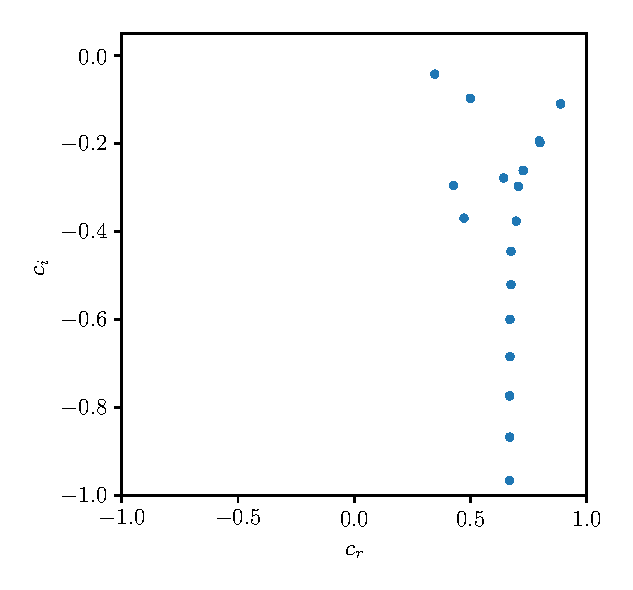
\includegraphics[width=60mm]{figures/pR=1000a=1M=200order=2.eps}
    }
    \subfloat[$ R = 7500$]{
        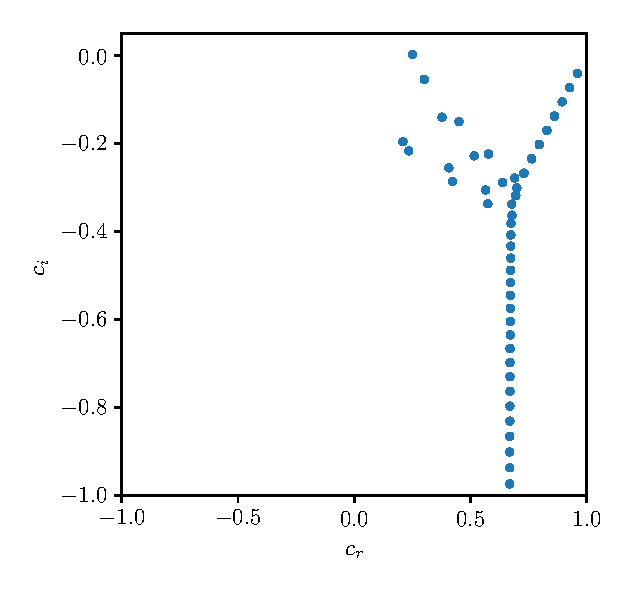
\includegraphics[width=60mm]{figures/pR=7500a=1M=200order=2.eps}
    }
    \caption{Eigenvalue spectra for a stable Poiseuille flow ($R = 1000$) and an unstable flow ($R = 7500$}
    \label{fig:unstablevstableflow}
\end{figure}

The spectrum for $ R = 10000$ and $ M = 200 $ can be seen in Figure \ref{fig:r10000} and forms a 'Y' shape. This is a classic case when it comes to Poiseuille flow and this spectrum matches those seen in papers such as \citet{dongarra1996chebyshev, bukhari1997spectral, antar1976eigenvalue}. We can see that there are 3 distinct 'families' of eigenvalues. The bottom straight line is referred to as the S family and contains a pattern of alternating odd and even eigenvalues \citep{dongarra1996chebyshev}, the top right branch is referred to as the P family and consists of overlapping pairs of odd and even eigenvalues \citep{dongarra1996chebyshev} and the 'spray' of eigenvalues forming the left branch is referred to as the A family of eigenvalues. These names come from \citet{mack1976numerical}.

\begin{figure}[h!]
    \centering
    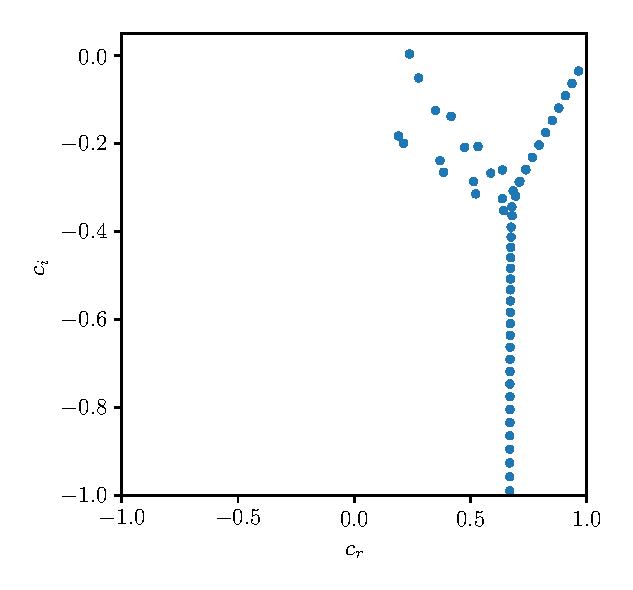
\includegraphics[width=80mm]{figures/pR=10000a=1M=200order=2.eps}
    \caption{Eigenvalue spectra for plane Poiseuille flow with $ R = 10000 $}
    \label{fig:r10000}
\end{figure}

We can see that Poiseuille flow is unstable at $ R = 10000$ because there is one 'critical eigenvalue' that has an imaginary part just slightly above $ 0 $. This is consistent with what other papers have found, most notably \citet{orszag1971accurate}. We will discuss how accurately the different methods reproduce the value of this critical eigenvalue in Section \ref{section:p_comparison}.

Finally, we should verify that all three of our methods produce similar results. Figure \ref{fig:comparison_poiseuille} shows a comparison between all three methods for Poiseuille flow at $ \al = 1 $, $ R = 10000 $ with $ 200 $ polynomials ($ M = 200$). As can be seen, the spectra all look similar, showing that the methods appear to be consistent. However, there are significant differences between these methods which can become more pronounced at higher and lower values of $ R $ and $ M $. A more thorough comparison is the focus of Section \ref{section:p_comparison}.

\begin{figure}[h!]
    \centering
    \subfloat[Fourth order spectrum]{
        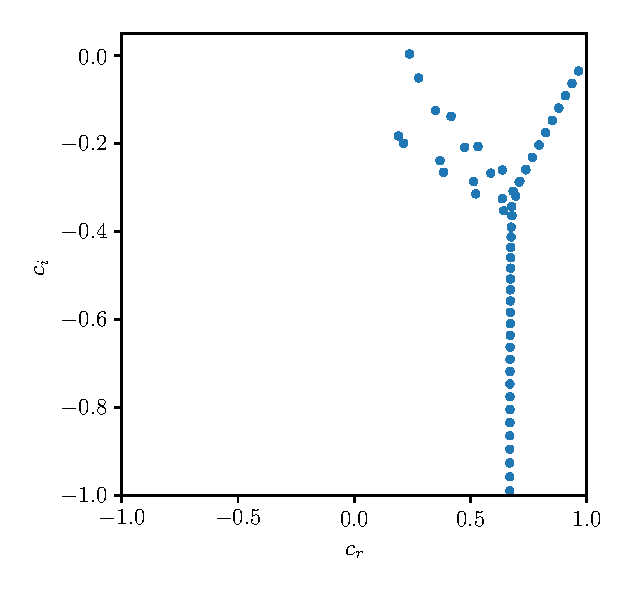
\includegraphics[width=50mm]{figures/p_flow_order_4_10000.eps}
    }
    \subfloat[Second order spectrum]{
        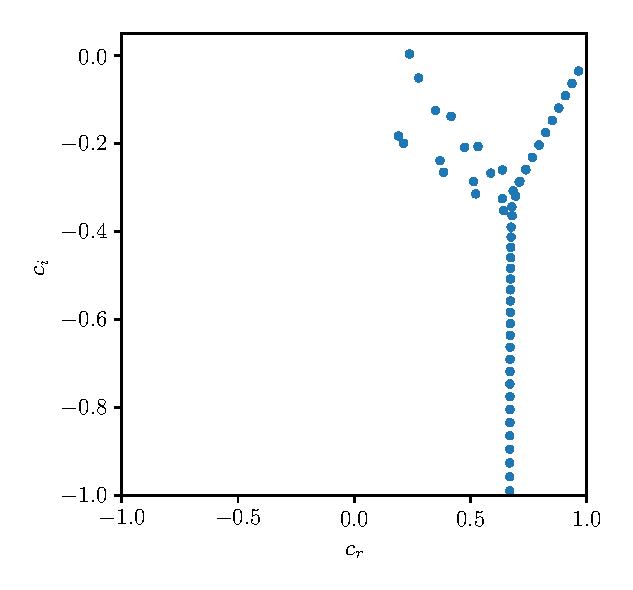
\includegraphics[width=50mm]{figures/p_flow_order_2_10000.eps} 
    }
    \subfloat[First order spectrum]{
        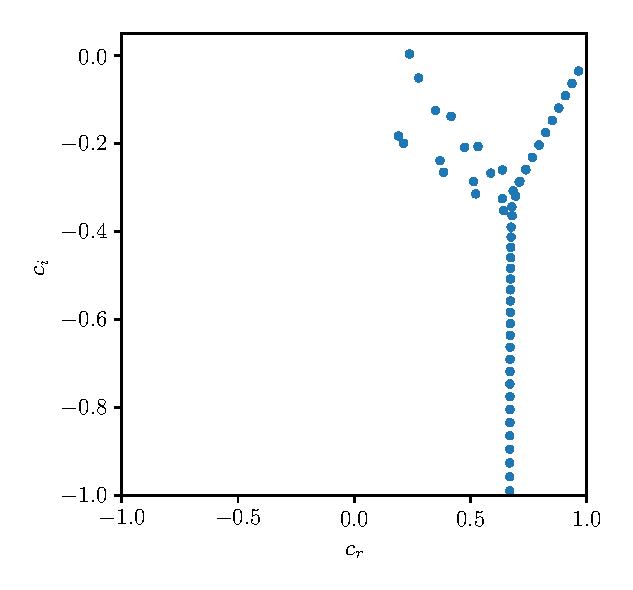
\includegraphics[width=50mm]{figures/p_flow_order_1_10000.eps}
    }
    \caption{The spectrum of Poiseuille flow for $ \al = 1 $, $ R = 10000 $ using different orders of method. They are consistent with each other which implies that these methods all work well for this value of $ R $.}
    \label{fig:comparison_poiseuille}
\end{figure}

\section{Basic results - Couette Flow}

If we run the second order method for Couette flow with $R = 8000$, $M = 200$ we get the spectrum shown in Figure \ref{fig:couettebroken}. However there is an obvious discrepancy in the spectrum when compared to the one in papers such as \citet{bukhari1997spectral}, the spectrum is not symmetric. 

\begin{figure}[h!]
    \centering
    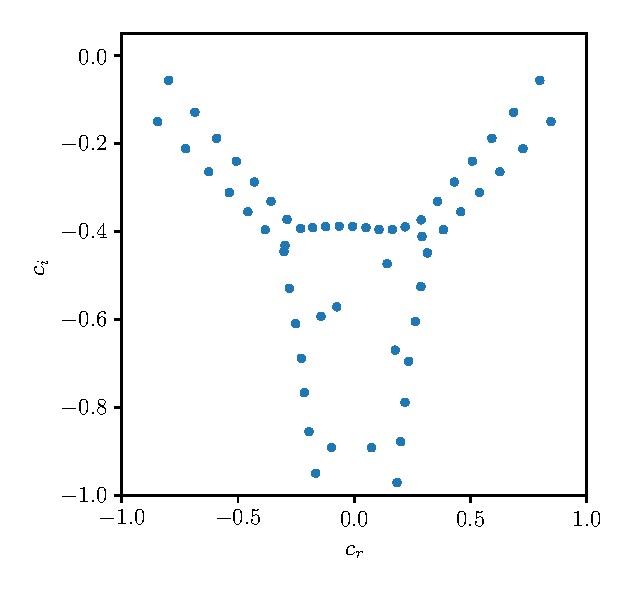
\includegraphics[width=80mm]{figures/couette_broken.eps}
    \caption{Spectrum of Couette flow with $ R = 8000$. There are some interesting discrepancies in this spectrum}
    \label{fig:couettebroken}
\end{figure}

It turns out this is due to the boundary conditions we have used causing numerical error. As noted in \citet{canuto2007spectral} in the case of plane channel flow, the odd and even terms in the sums representing our boundary conditions can be decoupled. This leaves us with an alternative set of boundary conditions
\begin{equation}
    \sum^M_{\substack{k = 0 \\ k \equiv 0 \ (\text{mod } 2)}} a_k =  \sum^M_{\substack{k = 1 \\ k \equiv 1 \ (\text{mod } 2)}} a_k = \sum^M_{\substack{k = 0 \\ k \equiv 0 \ (\text{mod } 2)}} k^2 a_k = \sum^M_{\substack{k = 1 \\ k \equiv 1 \ (\text{mod } 2)}} k^2 a_k = 0.  
\end{equation}

The first two conditions here correspond to the boundary conditions on $ \p(z)$, while the second two correspond to the boundary conditions on $ \p'(z) $. Using these alternative boundary conditions again with $ R = 8000$, $ M = 200 $ produces the spectrum seen in Figure \ref{fig:couette_fixed}. As can be seen, the result is now symmetric which fits the spectra seen in other literature such as \citet{bukhari1997spectral, DONGARRA1996399}.

The reason why these boundary conditions fix the spectrum is a little unclear. The most likely is due to the very large range in values in the matrices caused by the $ (-1)^k k^2$ in the original boundary conditions causing additional numerical error.

\begin{figure}[h!]
    \centering
    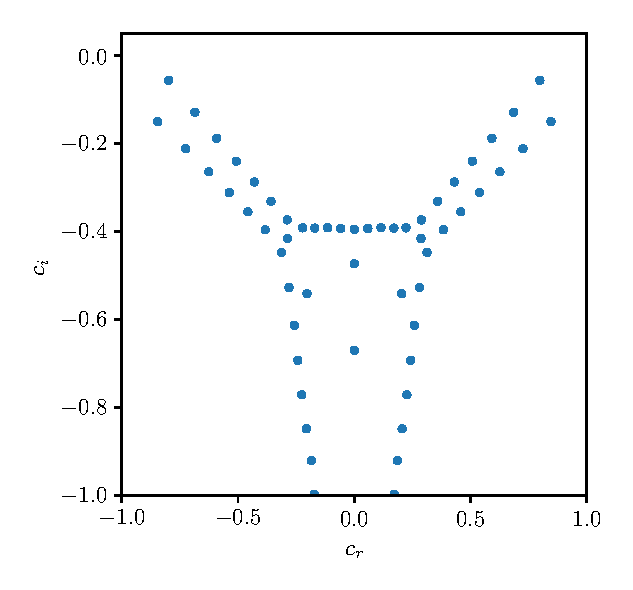
\includegraphics[width=80mm]{figures/couette_fixed.eps}
    \caption{Spectrum for Couette flow with $ R = 8000$ with alternative boundary conditions. The discrepancies seen in Figure \ref{fig:couettebroken} are not present here} 
    \label{fig:couette_fixed}
\end{figure}

If we look at Figure \ref{fig:couette_fixed}, we can see that Couette flow appears to be stable for this value of $ R$. If we test other values of $ R$ too, we find that Couette flow is stable for all values of $R$. This matches the findings of \citet{bukhari1997spectral} and other literature.

It turns out that these methods only work for very low $ R$ in the case of Couette flow. As seen in \citet{dongarra1996chebyshev}, all Couette flow spectra should look similar to the spectrum shown in Figure \ref{subfig:couette_3000}, with a single straight tail at around $ c_r = 0 $ that splits two symmetric sprays of eigenvalues as $ c_i \to 0 $. \citet{DONGARRA1996399} observed divergence from this spectrum as early as $ R = 3500 $, which our program reproduces as seen Figure \ref{subfig:couette_3500}.

\begin{figure}[h!]
    \centering
    \subfloat[$R = 3000$, $ M = 200$]{
        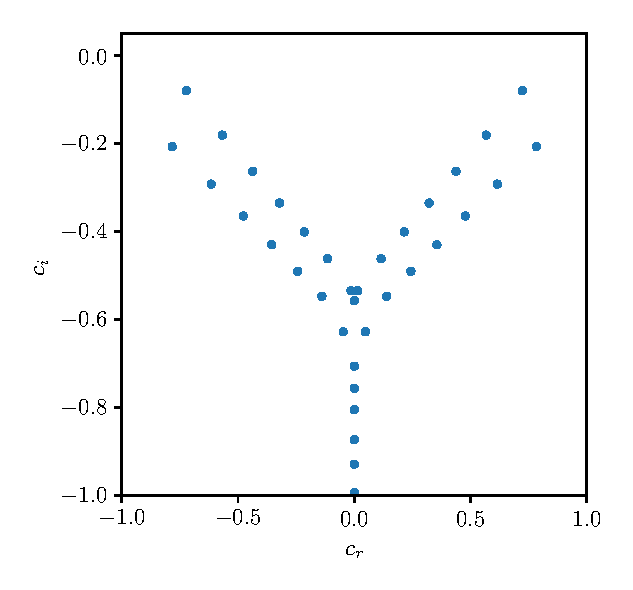
\includegraphics[width=60mm]{figures/couetteR=3000.eps} \label{subfig:couette_3000}
    }
    \subfloat[$R = 3500$, $ M = 200$]{
        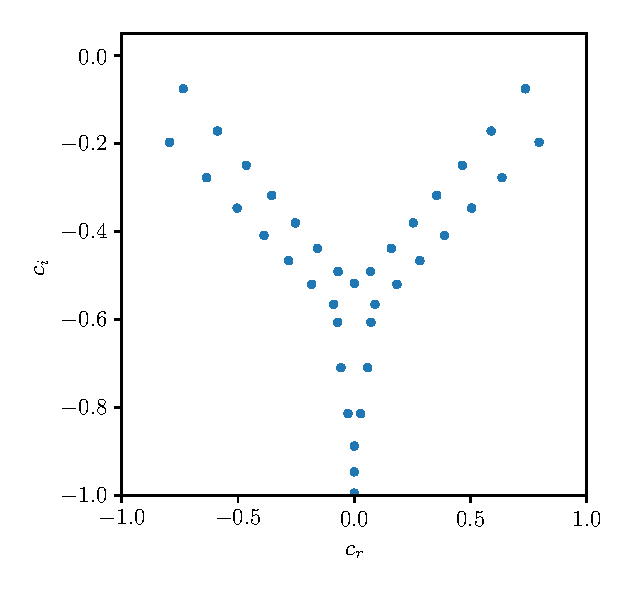
\includegraphics[width=60mm]{figures/couetteR=3500.eps} \label{subfig:couette_3500}
    }
    \caption{The spectrum of Couette flow with different values of $ R$. The left plot shows an expected plot, while the right plot shows a divergence from the expected spectrum.}
    \label{fig:couette_3000}
\end{figure}

A comparison between our three methods for Couette flow with $ R = 3000 $ with $ M = 200 $ is shown in Figure \ref{fig:comparison_couette}. As can be seen, unlike in the case of Poiseuille flow, the spectra produced vary significantly. The first order method looks the most accurate to the plot of $ R = 3000 $ in \citet{DONGARRA1996399} as expected, with the second order method looking extremely similar. On the other hand, the fourth-order method shows a significant divergence from the expected spectrum. This implies that the fourth-order method is not very good in the case of Couette flow.

\begin{figure}[h!]
    \centering
    \subfloat[Fourth order spectrum]{
        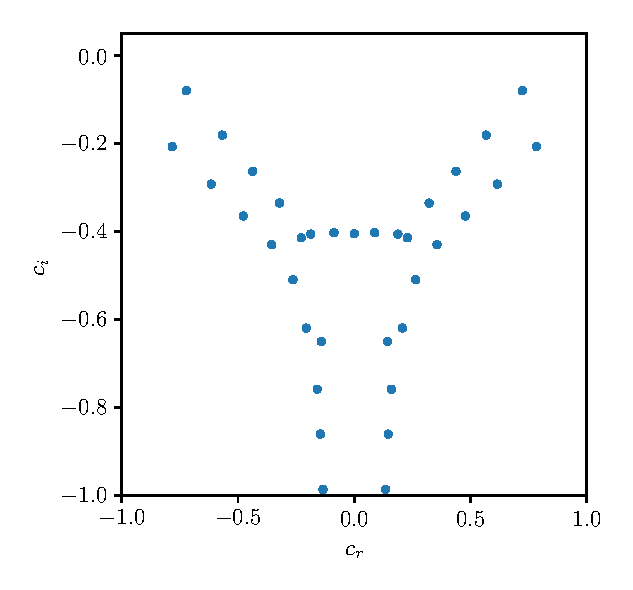
\includegraphics[width=50mm]{figures/c_flow_order_4_3000.eps}
    }
    \subfloat[Second order spectrum]{
        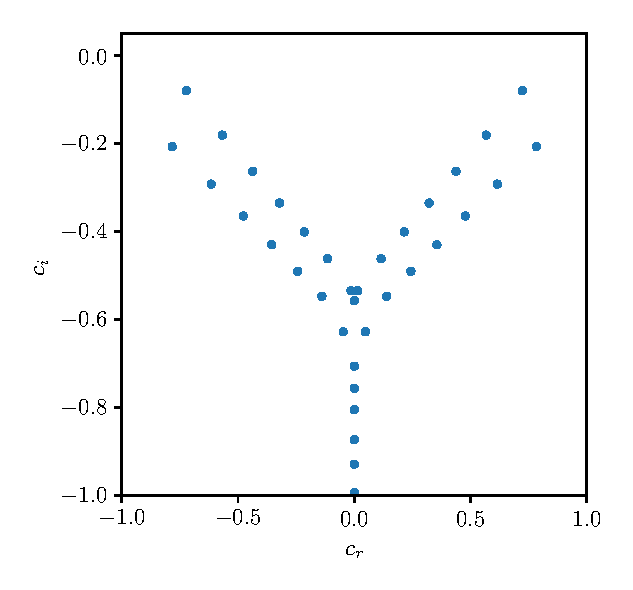
\includegraphics[width=50mm]{figures/c_flow_order_2_3000.eps} 
    }
    \subfloat[First order spectrum]{
        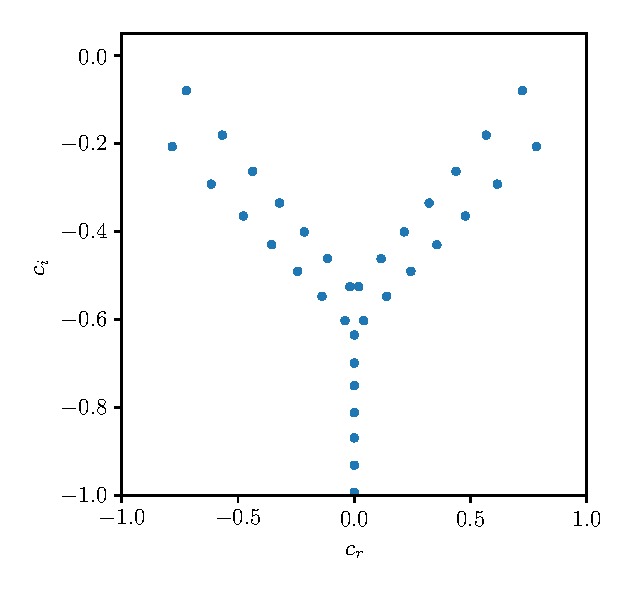
\includegraphics[width=50mm]{figures/c_flow_order_1_3000.eps}
    }
    \caption{The spectrum of Couette flow for $ R = 3000 $ using different orders of method. The fourth-order plot is significantly more diverged than the others, while the first-order method appears to be the most accurate.}
    \label{fig:comparison_couette}
\end{figure}

\citet{DONGARRA1996399} was able to get an accurate spectrum up until $ R = 13000$ by using $128$-bit floating point arithmetic rather than the $ 64$-bit arithmetic that our program uses. We can also reduce the divergence by tweaking the number of polynomials used. We will discuss this further in the next section where we compare the three different methods and their accuracy.

\section{Time Comparison of Methods} \label{section:time_comparison}

Now that we have verified the basic results of our program for both Poiseuille and Couette flow, we can move on to discussing how the $3$ different methods differ. There are advantages and disadvantages to each, so is there an obviously best choice? 

To start with let's compare perhaps the most obvious difference that we notice when running these programs, the difference in computation time. As mentioned in Chapter \ref{chap:numerics}, each method requires larger and larger matrices, and therefore more operations to both set up and solve. The Python program in Appendix \ref{code:timecomp} calculates the time taken for each method for different values of $M $. Figure \ref{fig:timecomp} shows the results of this program, a time comparison between the fourth-order method (green line), second-order method (orange line) and first-order method (blue line) for various values of $M$. 

As we can see there is a significant difference in the time taken for each of the methods, particularly between the first-order method and the other two methods. Even using just $ M = 200$ the first order method is significantly slower than the other two - taking over $2$ minutes to run at $M = 500$! This graph also highlights the main advantage of the fourth-order method, its speed. Notice also that while slower than the fourth order method, the second order method is still much faster than the first order method, taking less than $20$ seconds at $M = 500$. 

\begin{figure}
    \centering
    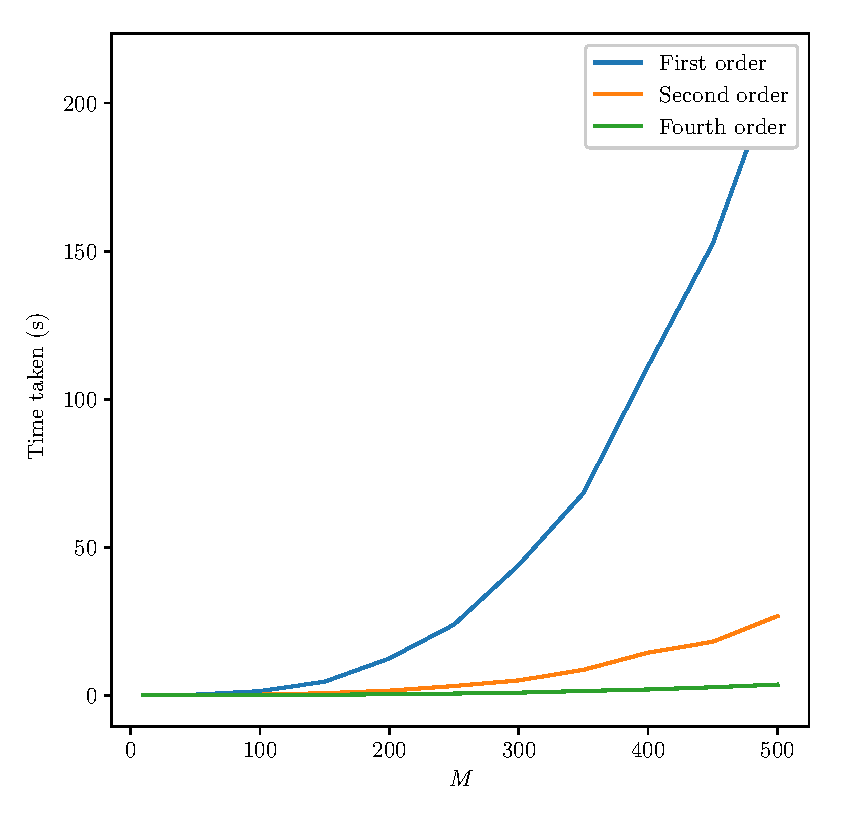
\includegraphics[width=100mm]{figures/time_comparison.eps}
    \caption{A comparison of times for the methods of different orders.}
    \label{fig:timecomp}
\end{figure}

So if the fourth-order method is that much faster than the other two methods, why bother using the others at all? The answer is due to the amount of accuracy that is lost at higher values of $ M $ or even $ R$. As we will see, each method of decreasing order is more accurate than the one before. But how does this inaccuracy present itself in the cases of Poiseuille and Couette flow? 

\section{Accuracy - Poiseuille Flow} \label{section:p_comparison}

To start with let's examine these methods in the case of Poiseuille flow. Figure \ref{fig:inaccdemo} shows eigenvalue spectra for the second order method run for $ R = 20000 $ with $ M = 150,\ 200,\ \text{and } 1000 $. The $ M = 200 $ plot looks as we would expect, but we see some interesting features in the $M = 150 $ and $ M = 1000 $ plot. 

\begin{figure}[h!]
    \centering
    \subfloat[$R = 20000,\ M = 150 $]{
        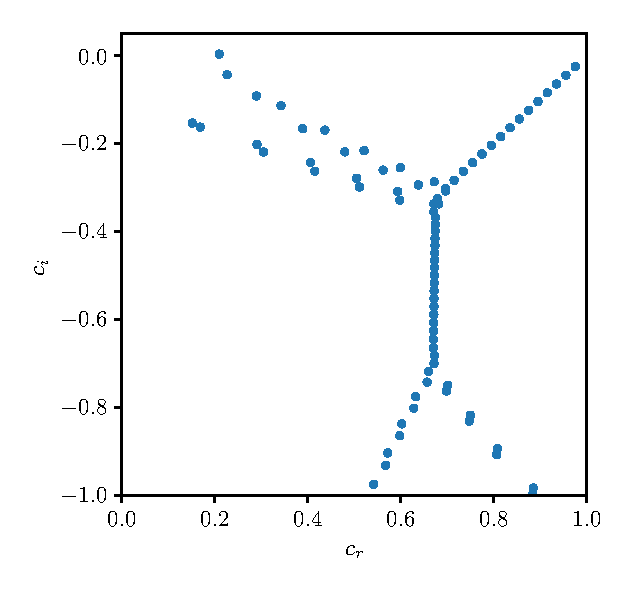
\includegraphics[width=50mm]{figures/pR=20000a=1M=150order=2.eps}
    }
    \subfloat[$R = 20000,\ M = 200 $]{
        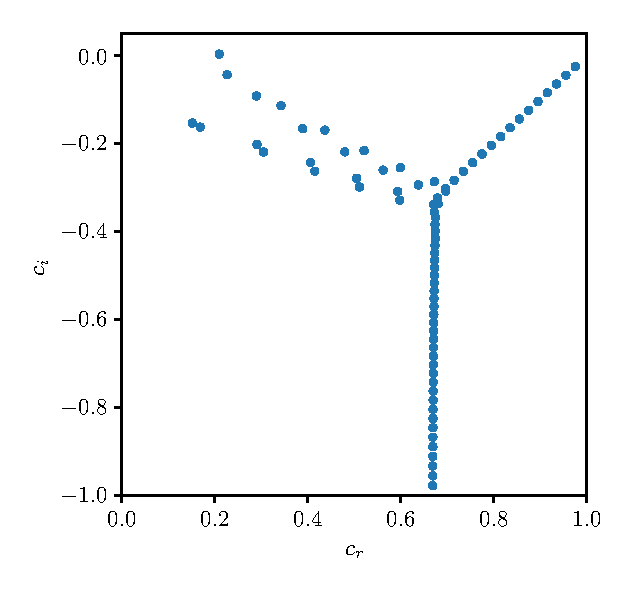
\includegraphics[width=50mm]{figures/pR=20000a=1M=200order=2.eps}
    }
    \subfloat[$R = 20000,\ M = 1000 $]{
        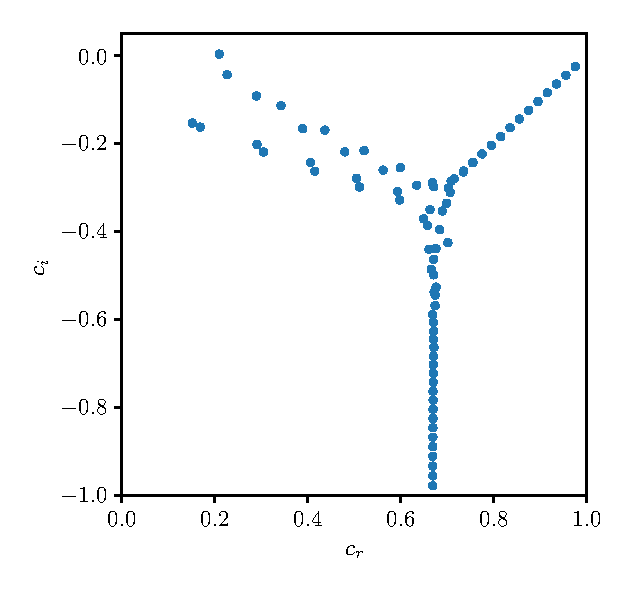
\includegraphics[width=50mm]{figures/pR=20000a=1M=1000order=2.eps}
    }
    \caption{Eigenvalue spectra for various values of $ M $ with $ R = 20000 $}
    \label{fig:inaccdemo}
\end{figure}

In the $M = 150 $ plot we can see a 'split' in the S family of eigenvalues. This tail is caused by using a number of polynomials that is too low to accurately determine eigenvalues with a lower imaginary part \citep{dongarra1996chebyshev}. In fact, if we extended the graph down on the $ M = 200$ and $M = 1000$ plots we would see a similar split. The reason that this isn't a concern is that we are concerned with the stability of the solution, and therefore care more about eigenvalues with imaginary parts that are close to $ 0$. The modes with eigenvalues with imaginary parts much below $0$ decay extremely fast and therefore are very stable.  

If we look at the $ M = 1000$ plot we can see a small triangle in the centre of the spectra, where the $3 $ branches meet. This is sometimes referred to as the 'triangle of instability' and is an indication that numerical error is present in the spectra \citep{dongarra1996chebyshev}. This occurs when either $ R$ or $ M $ is too high. We can use this to easily visualise the difference in numerical error between our different methods. Figure \ref{fig:trianglecomp} shows the spectra for $ R = 30000$ with $ M = 500$ generated by the fourth-order, second order and first-order methods respectively.

\begin{figure}[h!]
    \centering
    \subfloat[Fourth order]{
        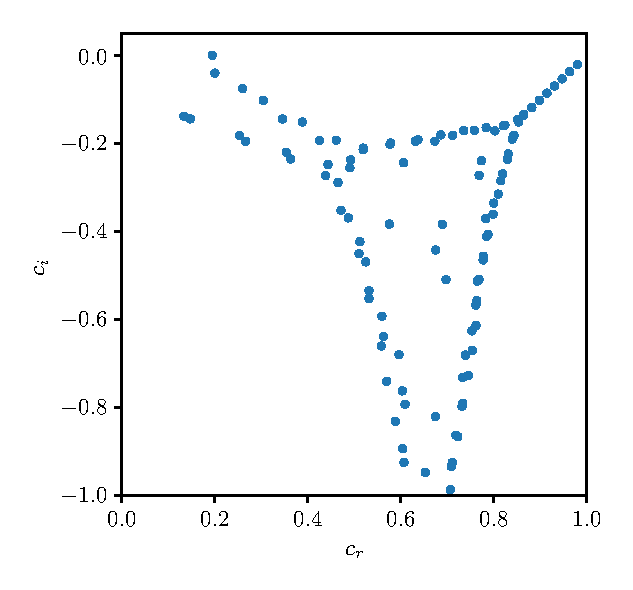
\includegraphics[width=50mm]{figures/pR=30000a=1M=500order=4.eps}
    }
    \subfloat[Second order]{
        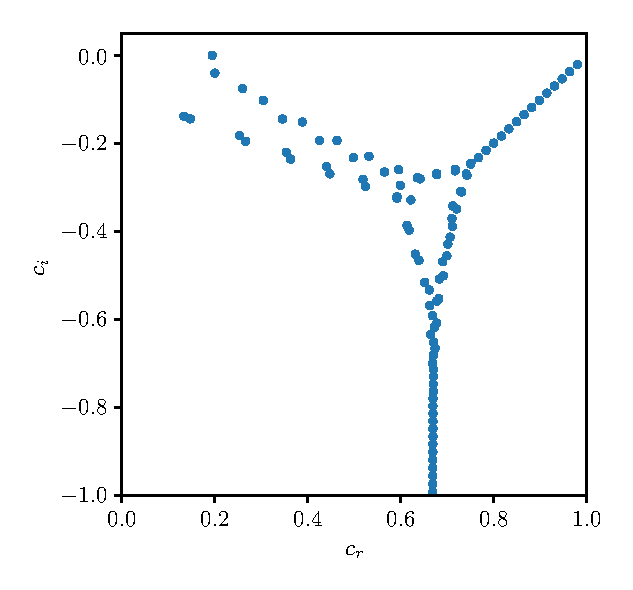
\includegraphics[width=50mm]{figures/pR=30000a=1M=500order=2.eps}
    }
    \subfloat[First order]{
        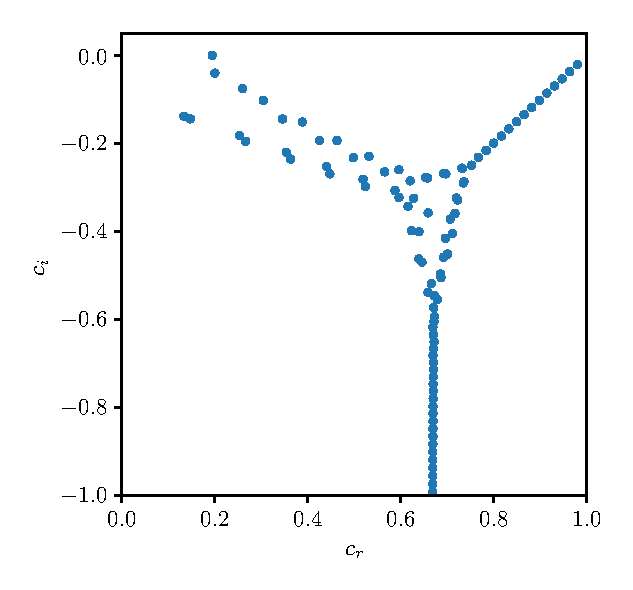
\includegraphics[width=50mm]{figures/pR=30000a=1M=500order=1.eps}
    }
    \caption{Eigenvalue spectra for $ R = 30000$, $ M = 500$ generated using methods of decreasing order (left to right)}
    \label{fig:trianglecomp}
\end{figure}

As can be seen, the difference in numerical accuracy between the fourth-order method (left spectrum) and second-order method (centre spectrum) is massive, the triangle of instability heads off of the bottom of the screen in this example. However while noticeable, the plots imply that the numerical error between the second-order method (centre spectra) and the first-order method (right spectra) is far less significant. This is an extreme example however, it turns out that the triangle of numerical error can never be removed from the spectrum of $ R = 30000$ no matter how high the number of polynomials used. A solution may be to use higher precision floating points, as \citet{dongarra1996chebyshev} show in the $ R = 28000$ case this can get rid of the triangle of instability altogether. 

This along with Figure \ref{fig:inaccdemo} imply two important things about these methods. First of all, the number of polynomials (value of $M $) chosen affects the accuracy of the produced spectra significantly. This must be remembered if the aim is to get an accurate representation of a specific portion of the spectra for a given value of $ R$. Secondly, if the value of $ R $ is high enough there is no way of completely removing the numerical instability. This implies that for high values of $R$, this method is not very useful for determining the eigenvalue spectrum. 

However, there is another more important way that numerical error can present itself. This is in the accuracy of the critical eigenvalue. This value must be computed accurately as it often has an imaginary part very close to zero and if computed incorrectly we could end up drawing the wrong conclusion about the stability of a flow.

\citet{orszag1971accurate} computed the critical eigenvalue for Poiseuille flow with $R = 10000$, $ \al = 1$ and (to 8 decimal places) found a value of 
\begin{equation}
     0.23752649 + 0.00373967i.
\end{equation} 

Table \ref{table:comparison} shows a side-by-side comparison of the critical eigenvalue produced by each method at different values of $M $ for Poiseuille flow with $ R = 10000$, $ \al = 1$. We can see a few interesting things here. First, all three methods obtain the correct eigenvalue at around $ M = 60$, though the first-order method produces the value accurately slightly earlier at around $M = 50$. Secondly, as $M $ gets larger the fourth-order and second-order methods lose accuracy. The fourth-order method is only accurate to 5 decimal places by the time $M = 200$, whereas the second-order and first-order methods are still accurate to 8 decimal places. By the time $M = 500$, the fourth-order method is only accurate to 4 decimal places. At this point, the second-order method has lost some accuracy and is now only accurate to 7 decimal places, but the first-order method is still accurate to 8 decimal places. This implies that the numerical error in the first-order method has a magnitude of less than $ 10^{-8}$ at $ M = 500$. This shows that the lower-order methods are indeed more accurate, as is expected with the tau method. 

\begin{table}[h!]
\centering
 \begin{tabular}{c | c | c | c} 
 M & Fourth-order & Second-order & First-order \\ [0.5ex] 
 \hline
 10 & 0.74378020+0.63468457i & 0.94669728+0.38207669i & 0.94669728+0.38207669i \\ 
 20 & 0.73281177+0.0921027i & 0.64429837+0.06460278i & 0.64429837+0.06460278i \\
 30 & 0.23690887+0.00365516i & 0.23757258+0.00374383i & 0.23747672+0.00364734i \\
 40 & 0.23752676+0.00373427i & 0.23752741+0.00374191i & 0.23752761+0.00373901i \\
 50 & 0.23752651+0.00373968i & 0.23752648+0.00373967i & 0.23752649+0.00373967i \\ 
 60 & 0.23752649+0.00373967i & 0.23752649+0.00373967i & 0.23752649+0.00373967i \\
 \vdots & \vdots & \vdots & \vdots \\
 200 & 0.23752588+0.00374036i & 0.23752649+0.00373967i & 0.23752649+0.00373967i \\
 \vdots & \vdots & \vdots & \vdots \\
 500 & 0.2374707+0.00378162i & 0.23752646+0.00373950i & 0.23752649+0.00373967i \\
 \end{tabular}
 \caption{Comparison of critical eigenvalue produced by each method for $ R = 10000 $ for increasing values of $ M $. }
 \label{table:comparison}
\end{table}

Let's examine the convergence of the first-order method more closely for values above $ M = 50$. Table \ref{table:firstorder} contains the critical eigenvalues produced by the first-order method for $ M $ between 50 and 120. We can see that for $ M > 70$, the first 11 decimals are the same. As the tau method is expected to converge as $M $ increases, we can confidently say that this is a more accurate value for the critical eigenvalue for Poiseuille with $ R = 10000 $. Our estimate for the critical eigenvalue to 11 decimal places is
\begin{equation}
    0.23752648882+0.00373967062i.
\end{equation}

\begin{table}[h!]
\centering
 \begin{tabular}{c | c} 
 M & Critical Eigenvalue - First-order \\ [0.5ex] 
 \hline
 50  & 0.23752648798891834+0.0037396745437875040i \\
 60  & 0.23752648882528551+0.0037396706118949263i \\
 70  & 0.23752648882056760+0.0037396706231014325i \\
 80  & 0.23752648882017588+0.0037396706228313510i \\
 90  & 0.23752648882049590+0.0037396706231066680i \\  
 100 & 0.23752648882102453+0.0037396706230743916i \\
 110 & 0.23752648882018287+0.0037396706236932730i \\
 120 & 0.23752648882051130+0.0037396706231617796i 
 \end{tabular} 
 \caption{Critical eigenvalues for the first-order method. }
 \label{table:firstorder}
\end{table}

It is difficult to confirm that this is definitely the critical eigenvalue of Poiseuille flow with $ R = 10000 $ to $ 11 $ decimal places since in other literature, the authors only attempt to reproduce the $ 8 $ decimal place value found by \citet{orszag1971accurate}. Still, \citet{bukhari1997spectral} found that error was lowest at around this range of $ M $ and this value does match the value given by \citet{orszag1971accurate} to $8$ decimal places. The author of this report believes that this is a more accurate eigenvalue than that found by \citet{orszag1971accurate}.

We can also see that there appears to be a 'sweet spot' for accurately determining the critical eigenvalue for all of our methods at around $ M = 60$. This is interesting because this value of $ M $ is too low to obtain the whole spectrum correctly. This means there is a trade-off between accurately determining the critical eigenvalue for a flow compared to getting more accurate results for other eigenvalues. The more eigenvalues we try and determine, the less accurate our value for the critical eigenvalue is.

However, for high values of $R$ the numerical error in the critical eigenvalue is too high and as such we get that after a certain point, all flows are computed to be stable. This is the case no matter the method. For example, when $ R = 35000 $, all of our methods return that the flow is stable. But, we know that flows above a certain critical value of $R$ are unstable from our analytical bounds derived in Chapter \ref{chap:suffcons}. This means that since we've found that Poiseuille flow is unstable for $ R = 10000$, it must also be unstable for $ R = 35000 $, indicating that our program is incorrect. This isn't a concern, however, as we can still search for the critical value of $R$ as it must be below $ 10000$, and our methods accurately determine the stability of flows for lower $R$ values. We will compute this value in Section \ref{section:crit_r}.


% Figure \ref{fig:criterrorcomp} shows a graph of the error in the critical eigenvalue for each method for different values of $\log M $. This is specifically for the $ R = 10000 $ case. The most noticeable thing here is that the fourth-order method never determines the value of the critical eigenvalue to particularly high accuracy, whereas the second-order and first-order methods correctly compute the critical eigenvalue to around 8 decimal places. Notice also that this graph implies that there is a 'best' value for $M$, after which numerical error sets in and the computed value diverges from the true value (our approximation should converge as $ M \to \infty$).

% \textbf{make this figure nicer and explain where this error comes from. also actually compute the best number of polys to use}

% \begin{figure}
%     \centering
%     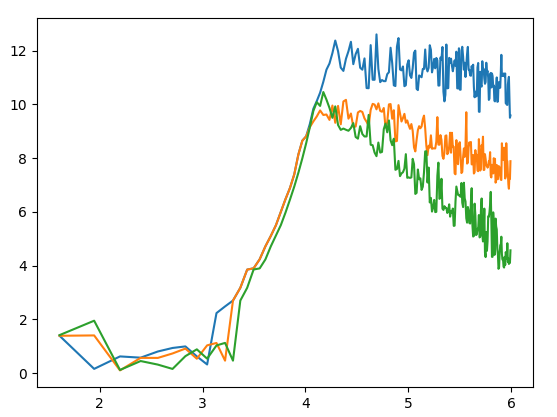
\includegraphics{figures/PlaceholderCritEigError.png}
%     \caption{Comparison of error between }
%     \label{fig:criterrorcomp}
% \end{figure}

% For both the second and first-order methods this peak occurs at around $M = 77  $, which agrees with \citet{dongarra1996chebyshev} who found that both these methods agree with the value \cite{orszag1971accurate} computed after this point. For $ R = 10000$ with $ 56 $ polynomials with both the second and first-order method, we find that the critical eigenvalue is (to $8$ decimal places)
% \begin{equation}
%     0.23752649 + 0.00373967 i,
% \end{equation}
% which agrees exactly with \citet{orszag1971accurate}. However, the peak for the first order method is an error of the magnitude of $ 10^{-13}$ which implies that we have an accurate value for this eigenvalue to $12 $ decimal places. This occurs at around $M = 75$. The produced critical eigenvalue for this value of $ M $ is (to $12 $ decimal places)
% \begin{equation}        0.237526488820+0.003739670623 i.
% \end{equation}

% It is difficult to confirm that this is definitely the critical eigenvalue of Poiseuille flow with $ R = 10000 $ to $ 12 $ decimal places, since in other literature the authors only attempt to reproduce the $ 8 $ decimal place value found by \citet{orszag1971accurate}. Still, \citet{bukhari1997spectral} found that error was lowest at around the same value of $ M $ and this value does match the value given by \citet{orszag1971accurate} to $8$ decimal places. It is likely that this value is correct to a slightly lower number of decimal places ($ 10 $ or $11$) as the method used to calculate the error, in this case, was fairly crude. The author of this report believes that a good case can be made that this is a more accurate eigenvalue than that found by \citet{orszag1971accurate}.

 % Despite the significantly higher accuracy of the first order of the second order method, the second order method still reaches an accuracy of $ 8 $ decimal places It is for this reason that the second order method is the most commonly used, since it offers significantly higher numerical accuracy than the fourth order method while also being significantly faster than the first order method.

\section{Accuracy - Couette Flow}

Are the forms of error seen in Poiseuille also seen in the case of Couette flow? Figure \ref{fig:couette_inaccdemo} shows the spectra produced using the second-order method using different numbers of polynomials. We can see that in the low $M $ plot (Figure \ref{subfig:lowMcouette}) we have a split in the tail of the spectrum similar to the split seen in Poiseuille flow at low polynomial counts. This split gets larger as $ M $ gets lower. In the high $ M $ case (Figure \ref{subfig:highMcouette}) we can see that in the centre of the plot, the eigenvalues have spread out into a 'diamond' which is the same as the 'triangle of instability' that appears when the value of $M$ is too high with Poiseuille flow. The centre plot does not have these errors, which implies that similar to Poiseuille flow, there is a best number of polynomials required to get an accurate spectrum for Couette flow.

\begin{figure}[h!]
    \centering
    \subfloat[$R = 3000,\ M = 85 $]{
        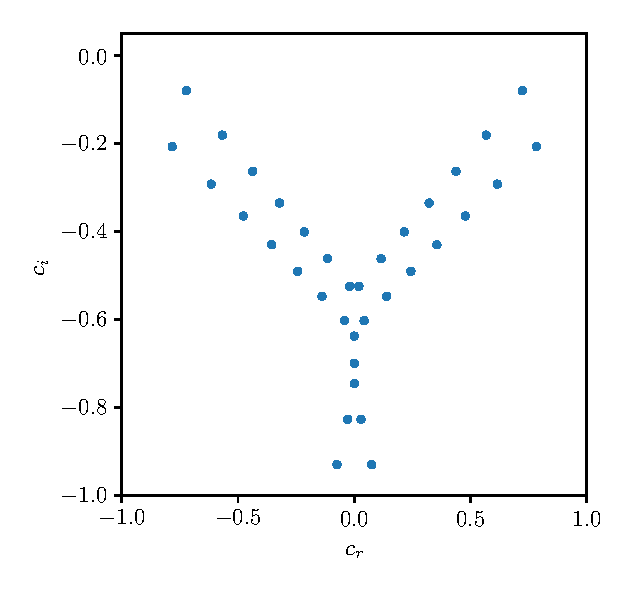
\includegraphics[width=50mm]{figures/c_flow_order_2_3000_M85.eps} \label{subfig:lowMcouette}
    }
    \subfloat[$R = 3000,\ M = 150$]{
        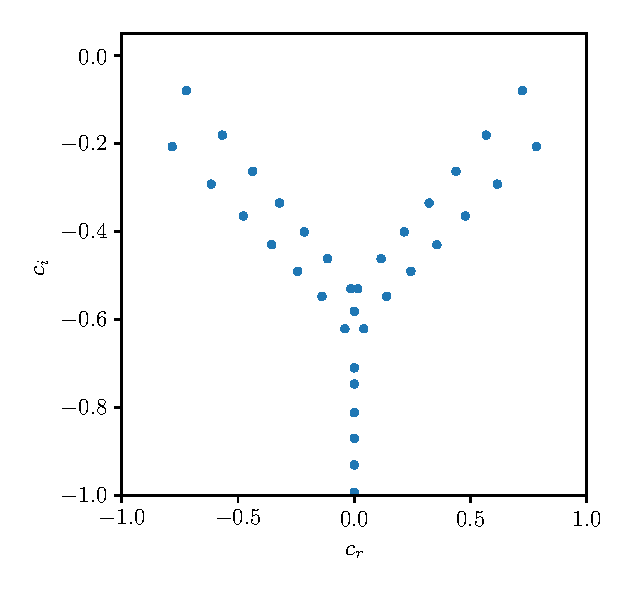
\includegraphics[width=50mm]{figures/c_flow_order_2_3000_M150.eps}
    }
    \subfloat[$R = 3000,\ M = 500 $]{
        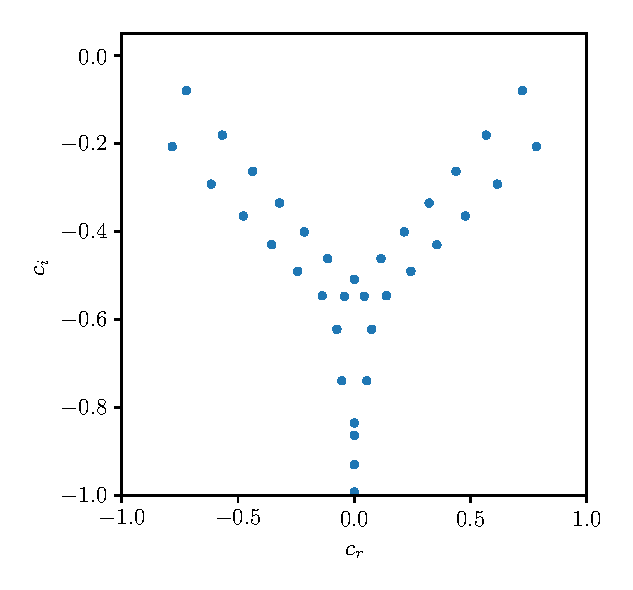
\includegraphics[width=50mm]{figures/c_flow_order_2_3000_M500.eps} \label{subfig:highMcouette}
    }
    \caption{Eigenvalue spectra for various values of $ M $ with $ R = 3000 $}
    \label{fig:couette_inaccdemo}
\end{figure}

This eigenvalue method will always find that Couette flow is stable, which is the expected result \citep{DONGARRA1996399}. This means that there is no 'critical eigenvalue' that we would particularly like to determine and test. We have also already seen in Figure \ref{fig:comparison_couette} that there is a significant difference in the results given based on the order of method used. This indicates that despite its significantly slower computation time, the best method for Couette flow is the first-order method.

\section{Eigenfunction - Poiseuille flow}

One of the key advantages of using the QZ algorithm to solve our system is that we can get the eigenvectors of our system extremely easily, as they are calculated during the process of calculating the eigenvalues \citep{moler1973algorithm}. However, in the case of the first and second-order systems, only the first $ M + 1$ entries correspond to our function $\phi$ and the remaining entries correspond to various derivatives of $\phi$. This means that our eigenfunction is found in this section of the eigenvector.

To get the eigenfunction from this eigenvector recall that the $k$th element corresponds to the coefficient of the $k$th order Chebyshev polynomial. Therefore to calculate our eigenfunction all we have to do is multiply each element by its corresponding Chebyshev polynomial.

Figure \ref{fig:eigenfunction} shows the eigenfunction of the critical mode for plane Poiseuille flow with $ R = 10000$,  $ M = 200 $. In this plot, the eigenfunction has been normalised so that it takes the value $ \phi = 1 + 0i $ at $ z = 0$ as in \citet{thomas1953stability}. The function is symmetric which is expected since the critical mode for plane Poiseuille flow is an even mode. The section of the graph with $ z > 0 $ also looks identical to the graph in \citet{drazin2004hydrodynamic} of the eigenfunction computed by \citet{thomas1953stability}, with one notable difference - the imaginary part is negative in Figure \ref{fig:eigenfunction} whereas, in Drazin and Reid, it is positive. This is because Thomas computed his eigenvalue with a different sign. This also explains why his critical eigenvalue has a negative imaginary part rather than the more common positive imaginary part.

\begin{figure}[h!]
    \centering
    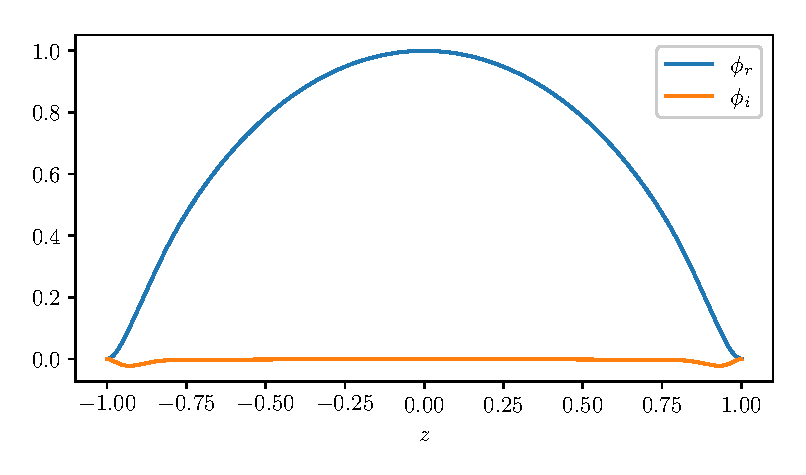
\includegraphics[width=130mm]{figures/eigenfunction.eps}
    \caption{The eigenfunction for the critical mode for plane Poiseuille flow. $ \phi_r $ is the real part and $\phi_i $ is the imaginary part.}
    \label{fig:eigenfunction}
\end{figure}

We can also see that this eigenfunction satisfies the boundary conditions of the Orr-Sommerfeld equation, as it is zero at the boundaries. However, we should also check the derivative of the eigenfunction is zero at the boundaries so that all boundary conditions are satisfied. Using the first order method, all we need to do is to pick the part of the eigenvector corresponding to $ \p_2$ as this is equivalent to $ D \p$. Figure \ref{fig:eigenfunction_diff} shows the plot of this (not normalised). As can be seen, it is zero at the endpoints, showing that all four boundary conditions have been satisfied!

\begin{figure}
    \centering
    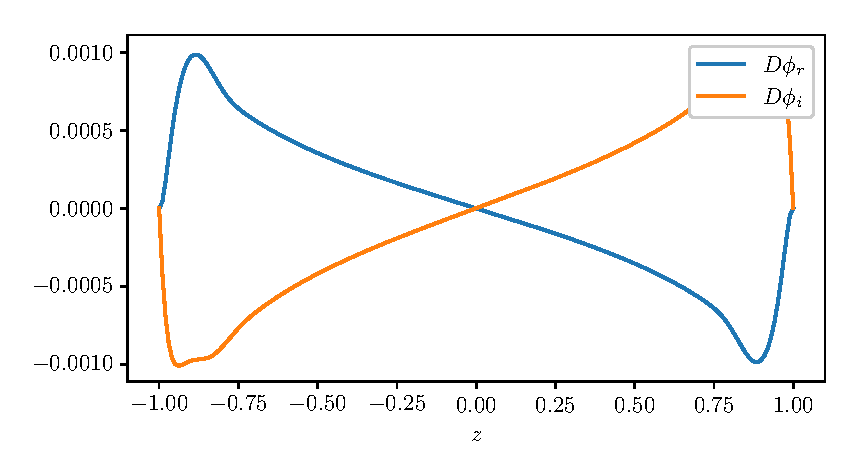
\includegraphics[width=130mm]{figures/eigenfunction_diff.eps}
    \caption{The un-normalized derivative of the eigenfunction for the critical mode of plane Poiseuille flow with $ R = 10000 $ and $ M = 200 $}
    \label{fig:eigenfunction_diff}
\end{figure}

We can take this eigenfunction a little further by computing $ \psi'(z) $, the streamfunction solution we took in Chapter \ref{chap:governing} (equation \eqref{streamfunction}) to get the Orr-Sommerfeld equation. Recall that 
\begin{equation}
    \psi'(x, z, t) = \p(z) \exp{i \alpha (x - c t)},
\end{equation}
where in this case, $ \alpha = 1$ and $ c$ is our critical eigenvalue.

Figure \ref{fig:streamfunction} shows the real part of the streamfunction for the eigenfunction in Figure \ref{fig:eigenfunction} plotted between $ 0 < x < 2 \pi$. As we would expect, it is periodic over this range.

\begin{figure}[h!]
    \centering
    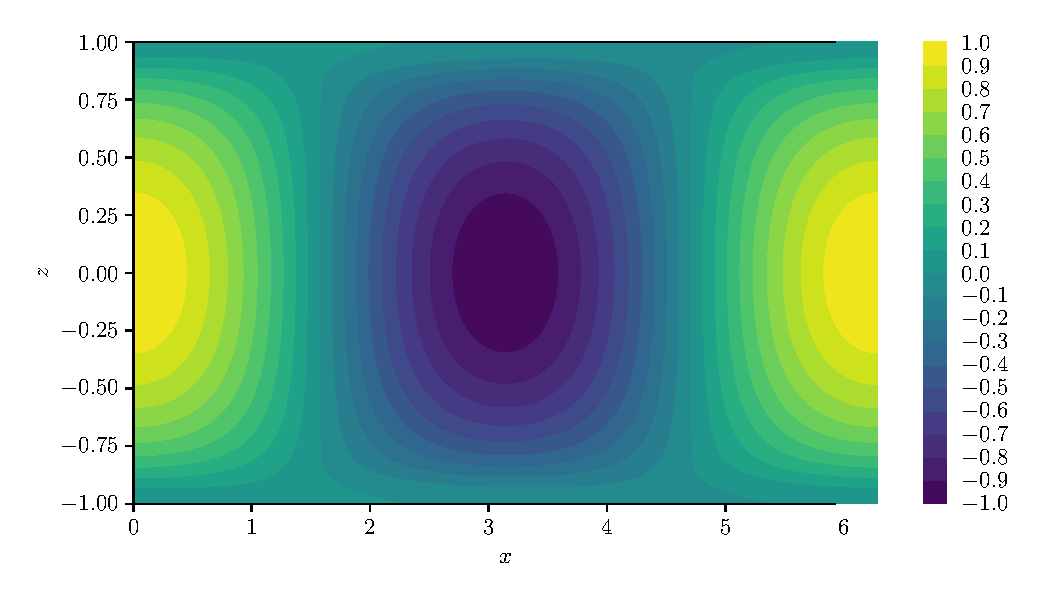
\includegraphics[width=150mm]{figures/streamfunction.eps}
    \caption{The real part of streamfunction for the critical mode of plane Poiseuille flow with $ R = 10000 $ and $ M = 200$}
    \label{fig:streamfunction}
\end{figure}

Code for the eigenfunction plot can be found in Appendix \ref{code:eigenfunction}, and for the streamfunction plot can be found in Appendix \ref{code:streamfunction}.

We can now move on to the most significant result this method can calculate, the critical Reynolds number for Poiseuille flow.

\section{Critical Reynolds Number - Poiseuille flow} \label{section:crit_r}

For a given $ \al$, we can compute the Reynolds number at which the corresponding mode becomes unstable (i.e. the imaginary part of the critical eigenvalue hits $ 0$). We can use this to plot a curve of marginal stability which provides a bound on stability in the same way that the analytic results from \citet{joseph1968eigenvalue, synge1938hydrodynamical} did. The Python program in Appendix \ref{code:criticalR} calculates these values of $ R $ using a bisection technique. The result of this program is shown in Figure \ref{fig:marg_curve}. Notice it takes a very similar shape to Joseph and Synge's bounds, with the unstable $ R$ value appearing to head to infinity as $ \alpha \to 0$ and as $ \alpha \to \infty$. However, the values of $R$ found are much higher than those given by Joseph and Synge. This is likely because the analytic bounds were calculated by significant approximations, and are therefore extremely inaccurate compared to our numerical method.

\begin{figure}[h!]
    \centering
    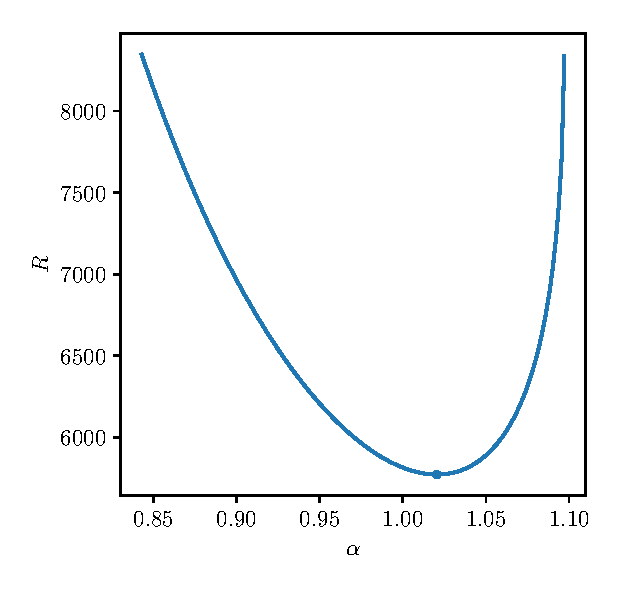
\includegraphics{figures/marginal_stability_curve.eps}
    \caption{The marginal stability curve for Poiseuille flow. The dot indicates the point of critical $R $ and $ \alpha$}
    \label{fig:marg_curve}
\end{figure}

We have a minimum point marked on the graph as a dot. This minimum corresponds to the famous \emph{critical Reynolds number}, the Reynolds number above which Poiseuille flow is unstable. The program computes this by recursively searching for the smallest value near the minimum point. To $6$ significant figures, the first order method with $ 50 $ polynomials finds
\begin{equation}
    R = 5772.22,\ \text{ at } \alpha = 1.02055,
    % R = 5772.221739281689,\ \text{ at } \alpha = 1.0205472421646122
\end{equation}
which matches the findings of \citet{orszag1971accurate}, who found that the first unstable mode of plane Poiseuille flow occurs at $ R = 5772.2 $ with $ \alpha = 1.02056 \pm 0.00001 $.

A value for the critical Reynolds number for Couette flow does exist, at about $ R = 45000 $ \citep{bukhari1997spectral}. Unfortunately, we cannot reproduce this value using this program as accuracy is lost so fast as $ R $ increases with Couette flow. Interestingly, \citet{bukhari1997spectral} quotes a slightly lower value for plane Poiseuille flow, although this doesn't seem to be supported in other literature, and our program cannot reproduce this value either.

These results differ significantly from those predicted by our analytic bounds from Chapter \ref{chap:suffcons}. The critical Reynolds number computed numerically is much higher for Poiseuille flow than the value obtained analytically. Recall that Joseph's more accurate bound predicted a value of roughly $ 9 $! However, Joseph and Synge's bounds did expect that the critical Reynolds number would be found at a low wavenumber, which we have found to be the case.

% \section{Basic Results - Poiseuille Flow}
% We first run the $2$nd order method for Poiseuille flow using the standard differentiation matrices suggested by \citet{dongarra1996chebyshev} for $ \al = 1, R = 10000 $ with $ 200 $ polynomials. This produces the classic eigenvalue spectra for plane Poiseuille flow found in many papers.

% The spectra can be seen in Figure \ref{fig:r10000} and forms a 'Y' shape. We can see that there are 3 distinct 'families' of eigenvalues \citep{mack1976numerical}. The bottom straight line is referred to as the S family and contains a pattern of alternating odd and even eigenvalues \citep{dongarra1996chebyshev}, the top right branch is referred to as the P family and consists of overlapping pairs of odd and even eigenvalues \citep{dongarra1996chebyshev} and the 'spray' of eigenvalues forming the left branch is referred to as the A family of eigenvalues.
% \begin{figure}[h!]
%     \centering
%     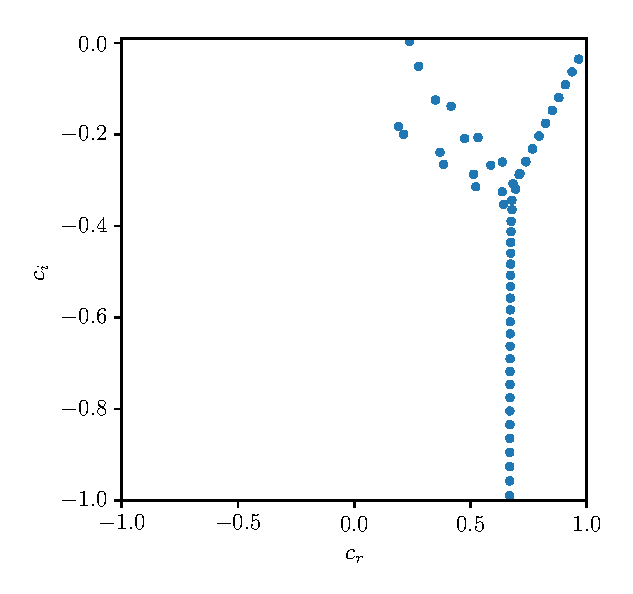
\includegraphics{figures/D2methodbig10000.eps}
%     \caption{Eigenvalue spectra for plane Poiseuille flow with $ \al = 1 $ and $ R = 10000 $}
%     \label{fig:r10000}
% \end{figure}

% We aim to reproduce the graphs seen in \citet{bukhari1997spectral} for the $ D^2 $ method. These all use $ \al = 1 $, $ 200 $ polynomials and $ R $ values between $ 5000 $ and $ 50000 $. We also include a graph of $ R = 100 $ and compare it to the graph found in \citet{antar1976eigenvalue}. 

% Note that the graph in \citet{antar1976eigenvalue} includes only the eigenvalues corresponding to the symmetric (even) modes (our program provides all the eigenvalues within the given range) and also that this graph has different limits on $ c_i $ to the other graphs.

% The spectra produced by our program can be seen in Figure \ref{fig:pspectra}. As can be seen, they match exactly with the graphs found in \citet{bukhari1997spectral, antar1976eigenvalue}. However, there is some interesting behaviour in the $ R = 30000 $ and $ R = 50000 $ cases. This is caused by either too few polynomials or numerical error and will be the focus of the next section where we analyse the accuracy of our various methods.
% \begin{figure}[p!]
%     \centering
%     \subfloat[$\al = 1 $ with $ R = 100 $]{
%         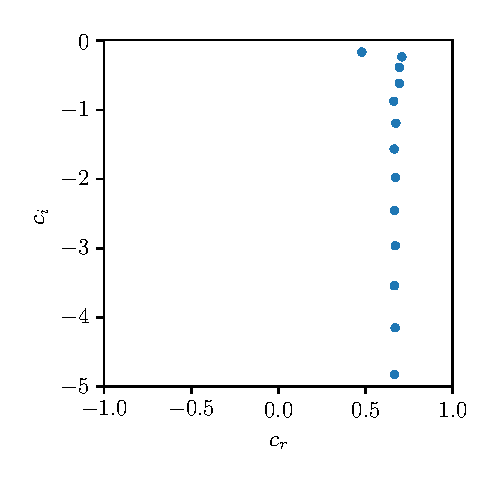
\includegraphics{figures/D2method100.eps}
%     }
%     \subfloat[$\al = 1 $ with $ R = 5000 $]{
%         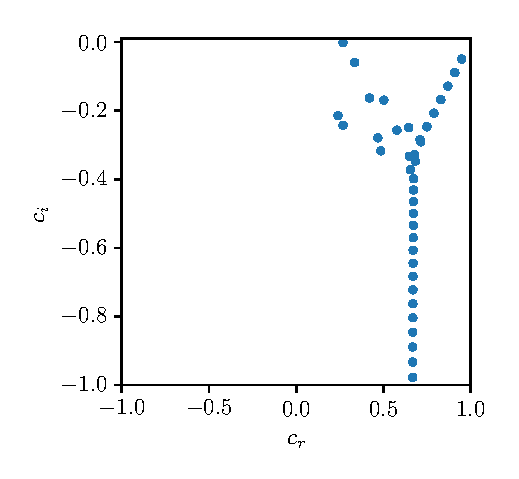
\includegraphics{figures/D2method5000.eps}
%     }
%     \hspace{0mm}
%     \subfloat[$\al = 1 $ with $ R = 7500 $]{
%         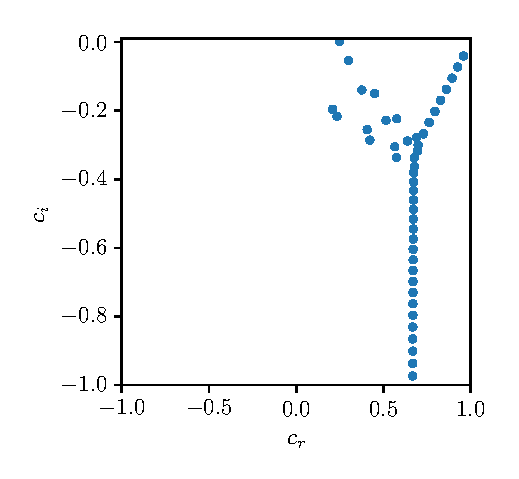
\includegraphics{figures/D2method7500.eps}
%     }
%     \subfloat[$\al = 1 $ with $ R = 10000 $]{
%         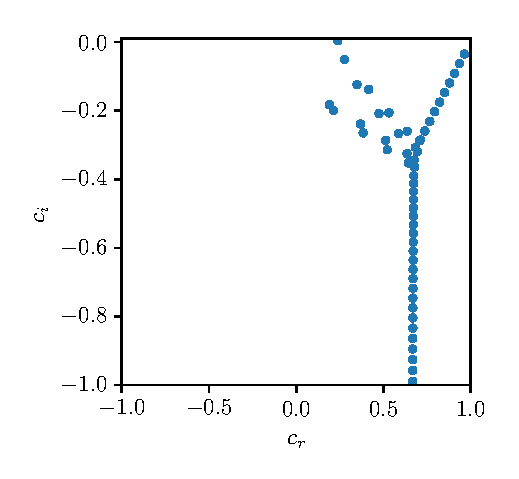
\includegraphics{figures/D2method10000.eps}
%     }
%     \hspace{0mm}
%     \subfloat[$\al = 1 $ with $ R = 30000 $]{
%         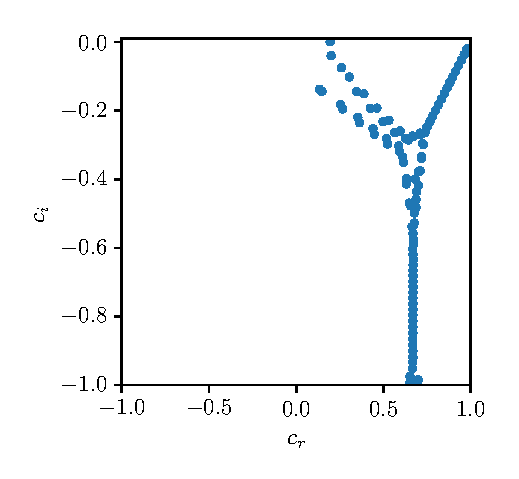
\includegraphics{figures/D2method30000.eps}
%     }
%     \subfloat[$\al = 1 $ with $ R = 50000 $]{
%         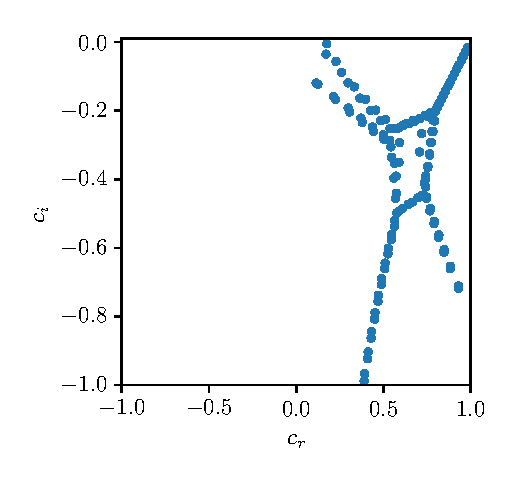
\includegraphics{figures/D2method50000.eps}
%     }
%     \caption{Graphs of the eigenvalue spectra for Poiseuille flow with $ \al = 1 $ and various values of $ R $}
%     \label{fig:pspectra}
% \end{figure}

% \textbf{discuss what values of polynomials are needed for this value to be found, e.g. for the 4th order case we cannot get the exact value as found by orszag} 

% \section{Basic Results - Couette Flow}

% \textbf{Show graphs of spectra}



% \section{Comparison and accuracy of methods}
% First we would like to compare the accuracy of our 4 different methods. To start we will examine the accuracy of just one method, the standard $2$nd order method. 

% Compare numerical accuracy, plots as in \cite{dongarra1996chebyshev} (triangle of numerical instability)

% Compare D4, D2, D1 methods. Compare both Poiseuille and Couette flow

% Plot curves of error for critical eigenvalue - a little cruder than some papers as Python returns eigenvalues in random order

% \textbf{comparision of time taken}

% \begin{figure}
%     \centering
%     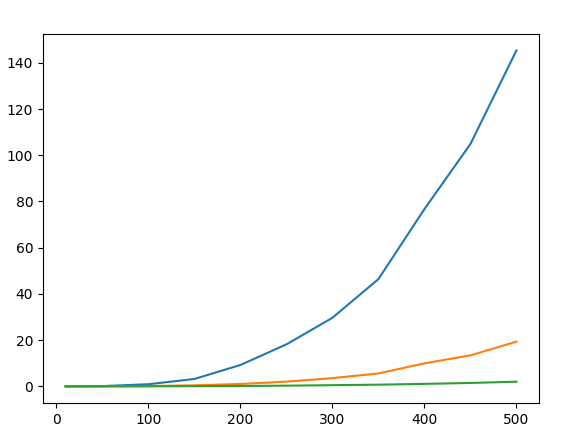
\includegraphics{figures/timecomp.png}
%     \caption{A comparison of time taken for various values of $M$ - PLACEHOLDER}
%     \label{fig:time_comp}
% \end{figure}


% \section{Critical Reynolds Number}

% curve of marginal stability
% compute for poiseuille and couette (if possible for couette)

% \section{Eigenfunction}

% Normalized the value at 0 to be $ 1 + 0 i $ as in \cite{thomas1953stability}, produces graph seen in \cite{drazin2004hydrodynamic}

% The program correctly produces an even eigenfunction, which is what we would expect

% % \section{Reynold's stress tensor}
% % As in \cite{drazin2004hydrodynamic}, \cite{stuart1966double}

% % \section{Stabilizing Poiseuille flow with Couette flow}
% % As \cite{potter1966stability, hains1967stability, reynolds1967finite}  

\chapter{Conclusion}
\label{chap:conc}

\section{Summary of results}
To conclude this report, let us summarise what has been shown. To begin, we introduced two classic types of plane flow, plane Poiseuille flow and plane Couette flow. We then used the governing equations for a plane channel flow to derive an important equation for linear stability, the Orr-Sommerfeld equation. The important parameters of the Orr-Sommerfeld equation were the Reynolds number $R$, the wavenumber $\al$ and its complex eigenvalue $ c$. From examining the Orr-Sommerfeld equation, we determined a flow must be unstable if it has an eigenvalue with an imaginary part greater than $0$.

From here we derived a few analytic bounds on the stability of a flow, the bounds first derived by \citet{synge1938hydrodynamical} and then the improved bounds derived by \citet{joseph1968eigenvalue, joseph1969eigenvalue}. When compared, Joseph's bounds had a higher minimum point (critical $R$ value) than Synge's bounds. From this, we can conclude that a more accurate bound on stability would likely have a larger critical $ R$ value since these bounds were extremely approximate. To get a better bound on stability and to enable us to test whether a flow is stable for a specific value of $R$, we turned to a numerical method based on Chebyshev polynomials.

We showed that not only do Chebyshev polynomials accurately approximate functions, but they also have several extremely useful recursive relations for their derivatives. These relations allowed us to represent the differentiation of a function by multiplying a vector of coefficients by a differentiation matrix. We also needed a way to represent the basic flow of plane Poiseuille and plane Couette flow, which was done by the  $P $ and $Q $ matrices of \citet{bukhari1997spectral}. We then showed that we could form a generalised eigenvalue problem by representing the whole fourth-order Orr-Sommerfeld equation using one matrix. However, as the matrix involved had terms that grew extremely fast we discussed two alternative methods. By splitting the Orr-Sommerfeld equation into two second-order differential equations or even four first-order differential equations, represented in a block matrix form. These two additional methods had matrices with slower-growing elements, and therefore higher numerical accuracy. To solve our eigenvalue problem, we implemented these methods in Python and used the implementation of the QZ algorithm of \citet{moler1973algorithm} to get our system's eigenvalues.

When applied to Poiseuille flow, all of the methods were able to produce consistent spectra in classic cases with $R< 10000$. From these spectra, we were able to determine that for low values of $R$, Poiseuille flow is stable, whereas it is unstable for $R$ larger than a certain critical value. Both the first and second-order methods were able to reproduce the value for the critical eigenvalue as calculated by \citet{orszag1971accurate}, however, the fourth-order method was unable to produce this value at any point.

When applied to Couette flow, we observed a large difference in the spectrum produced by each method, with the fourth-order method diverging particularly far from the expected spectrum. Each method was also significantly more sensitive to changes in the polynomial count.

In both cases, when $R$ or $M $ became large, a triangle (or diamond) of instability formed, showing that numerical error was present. While it was a smaller triangle for more accurate methods, for higher values of $R$ there was no value of $M$ for which the triangle disappeared. This indicates that these methods do not work very well for high $R$, i.e. less viscous fluids. We also observed that if the value of $M $ was too low, the eigenvalues lower down the spectrum (i.e. with imaginary parts much below zero) would split away from the straight branch expected. However, for determining the critical eigenvalue of a flow it was better to use a lower, but not too low value of $M$, to not lose accuracy to numerical error.

We then showed that our method can be used to calculate the eigenfunction for a flow. To verify this, we compared it with the computed eigenfunction for the critical mode of $R = 10000$, $ \al = 1$ of Poiseuille flow by \citet{thomas1953stability}. We verified that this eigenfunction does satisfy our boundary conditions, showing that it does satisfy both the Orr-Sommerfeld equation and its boundary conditions. We were also able to use this eigenfunction to get a streamfunction for this mode.

The final result of the report was a bound on stability computed using a bisection method. We were able to get that the critical Reynolds number for plane Poiseuille flow is $ R = 5772.22$ which matches up with the value found by \citet{orszag1971accurate}. While a critical value of $R$ for Couette flow has been mentioned in some literature such as \citet{bukhari1997spectral}, this could not be reproduced by our methods. Our method concluded that Couette flow is always stable which is the accepted norm as mentioned in \citet{trefethen1993hydrodynamic}.

\section{Application of Results}

How do these results relate to flows in the real world? The main conclusion we can draw is that for both Poiseuille and Couette flow, there appears to be a Reynolds number below which the flow is completely stable. We can use this to suggest possible ways in which a flow could be stabilised. For example, let's say we have Poiseuille flow in pipe flowing at a rate of 1 metre per second. Distilled water has a kinematic viscosity of about $ 1.0038e-006 $ metres squared per second at 20 degrees Celsius (from this table \href{https://www.engineersedge.com/fluid_flow/kinematic-viscosity-table.htm}{\textcolor{blue}{here}}). For this flow to have a Reynolds number below the critical value of 5772.22 we must have a characteristic length of below 0.00577222 metres or 5.77222 millimetres. If we recall the definition of the characteristic length in Chapter \ref{chap:governing} then we recall that this is half of the width of our channel i.e. its radius, implying that water flowing at a velocity of 1 metre per second at 20 degrees Celsius through a pipe with a radius of less than 5.77222 mm would be a stable Poiseuille flow.

If however, we were considering a flow of kerosene at the same speed and temperature, we would be able to pass it stably through a pipe with a radius of roughly 15.6 mm. This is because kerosene has a higher kinematic viscosity of around $2.71e-006$ metres squared per second.

Our method has shown that flows with a low Reynolds number are more stable than those with a high Reynolds number. We can therefore conclude that our three variables (characteristic velocity, characteristic length and kinematic viscosity) have the following effects on stability
\begin{enumerate}
    \item High-velocity flows are less stable than low-velocity flows,
    \item Flows travelling through a wide channel are less stable than flows travelling through a thin channel,
    \item Flows of high viscosity fluid are more stable than flows of low viscosity fluids.
\end{enumerate}

\section{Further Research}

The numerical method in this report is the Tau method of \citet{lanczos1988applied}. However, this was not the only method that we could have used. Another method is the Chebyshev collocation method. In this method, the points in both the differentiation matrices and the vectors are points in physical space \citep{canuto2007spectral}. While this method may seem more intuitive and therefore preferable, \citet{bukhari1997spectral} notes that this method cannot be used to represent diverging series, and can be more susceptible to round-off error if the problem is not well-posed. A proper comparison of these methods for the case of Poiseuille and Couette flow would have been interesting and would be a good next step for this project if it were to continue.

This numerical method can also be used to analyse more complex flows, such as a combination of Poiseuille and Couette flow and multi-layered analysis. In \citet{bukhari1997spectral}, these methods are used to solve problems in convection in magnetic and multi-layered cases. In \citet{antar1976eigenvalue}, the method is applied to another classic case, the Blasius boundary layer flow. Most flow profiles that satisfy the governing equations for plane channel flow can be used, as all that needs to be changed are the $ P $ and $Q$ matrices. 

Finally, a discussion of the significance of the critical Reynolds number is in order. As pointed out in \citet{trefethen1993hydrodynamic}, experimentally instability is seen at much lower Reynolds numbers than the critical Reynolds number would suggest. Both Couette and Poiseuille flow show instability at $R$ values in the hundreds in experiments. When considering a culprit for this inaccuracy, our first thought would be that these bounds were on linear stability, implying that maybe the non-linear terms are to blame for these instabilities. However, \citet{trefethen1993hydrodynamic} points out that these are non-modal instabilities and therefore the issue lies with the normal mode analysis and eigenvalue method itself. 



% \begin{itemize}
%     \item Summarize analytical findings
%     \item Summarize the advantages and disadvantages of each numerical method
%     \item Discuss Tau vs Collocation methods
%     \item Discuss the significance of $R_\text{crit}$ \cite{trefethen1993hydrodynamic}, \cite{schmid2002stability}
%     \item Discuss applications of these methods to more complex stability analyses such as
%     \begin{itemize}
%         \item Stability analysis of multilayered flow
%         \item Blasius flow/jets
%     \end{itemize}
% \end{itemize}

\appendix

\chapter{Code}

These appendices contain all the code used to generate the figures and results seen throughout this project. Unless stated in the comments of the code, this code is the author's own work. Readers interested in running the code themselves can find it in the following  \href{https://github.com/OscarRummery/projectIV}{\textcolor{blue}{GitHub repository}}.

The code listed is not necessarily in the order it was used in the text. A recommended starting point is to run the \codeword{tau\_tester.py} program in Appendix \ref{code:tautester} which will allow you to test all three methods of different orders and will also return the critical eigenvalue for a given flow.

\section{.eps Saver}
This is just a simple program used to save the plots generated as .eps files. A lot of the programs use this code to display the results, and as such anyone wishing to run these needs to have \LaTeX installed on their machine. 

\lstinputlisting{code/epssaver.py}
\newpage

\section{Chebyshev Python Class} \label{code:chebyshevclass}
\lstinputlisting{code/chebyshev.py}
\newpage

\section{Chebyshev Plotter} \label{code:chebyshevplotter}
\label{code:chebyplotter}
\lstinputlisting{code/chebyshev_plotter.py}
\newpage

\section{Chebyshev Function Approximator} \label{code:funcapprox}
\lstinputlisting{code/function_approx.py}
\newpage

\section{Tau Matrices} \label{code:tau_matrices}
\lstinputlisting{code/tau_matrices.py}
\newpage

\section{Tau Method Class} \label{code:tauclass} 
\lstinputlisting{code/chebyshev_tau.py}
\newpage

\section{Fourth Order Method} \label{code:fourthorder}
\lstinputlisting{code/D4method.py}
\newpage

\section{Second Order Method} \label{code:secondorder}
\lstinputlisting{code/D2method.py}
\newpage

\section{First Order Method} \label{code:firstorder}
\lstinputlisting{code/D1method.py}
\newpage

\section{Tau Method Tester} \label{code:tautester}
\lstinputlisting{code/tau_tester.py}
\newpage

\section{Tau Method Time Comparison} \label{code:timecomp}
\lstinputlisting{code/time_comparison.py}
\newpage

% \section{Error In Critical Eigenvalue} \label{code:error}
% \lstinputlisting{code/crit_eig_error.py}
% \newpage

\section{Eigenfunction Computation} \label{code:eigenfunction}
\lstinputlisting{code/eigenfunction.py}
\newpage

\section{Streamfunction Computation} \label{code:streamfunction}
\lstinputlisting{code/streamfunction.py}
\newpage

\section{Critical Reynolds Number Computation} \label{code:criticalR}
\lstinputlisting{code/crit_R.py}


\bibliography{bib/references}
\end{document}